%# -*- coding:utf-8 -*-
\documentclass[12pt,aspectratio=169,mathserif]{beamer}		
%\documentclass[12pt,mathserif]{beamer}		
%设置为 Beamer 文档类型,设置字体为 10pt,长宽比为16:9,数学字体为 serif 风格
%\documentclass{beamer}

%%%%-----导入宏包-----%%%%
\usepackage{gdut}			%导入 GDUT 模板宏包
\usepackage{ctex}			%导入 ctex 宏包,添加中文支持
\usepackage{amsmath,amsfonts,amssymb,bm}   %导入数学公式所需宏包
\usepackage{color}			 %字体颜色支持
\usepackage{graphicx,hyperref,url}
\usepackage{metalogo}	% 非必须
\usepackage{multicol}
%% 上文引用的包可按实际情况自行增删
%%%%%%%%%%%%%%%%%%	


\beamertemplateballitem		%设置 Beamer 主题

%%%%------------------------%%%%%
\catcode`\。=\active         %或者=13
\newcommand{。}{.}				
%将正文中的“。”号转换为“.”。中文标点国家规范建议科技文献中的句号用圆点替代
%%%%%%%%%%%%%%%%%%%%%

% Bibliography settings 参考文献设置
\usepackage[style=ieee]{biblatex}
\setbeamertemplate{bibliography item}[text]


%\tiny\scriptsize\footnotesize\small\normalsize\large\Large\LARGE\huge\Huge   这些是调整字体大小的命令。

%%%%----首页信息设置----%%%%
\title[ 《铛铛支付》项目报告]{《铛铛支付》项目报告}
\subtitle{一个面向企业的兼信息展示,用户管理等的多功能支付平台}			
%%%%----标题设置


\date[Apr. 04 2024]{2024年4月29日}
\usepackage{datetime}
%%%%----机构信息
%\data[\currenttime]{\currenttime}

\author[杜家楷]{
	\large 杜家楷 \\\medskip
	%{\small \url{xuezheng@mail2.gdut.edu.cn}} \\
	%{\small \url{http://www.gdut.edu.cn/}}
}
%%%%----个人信息设置

\institute[IOPP]{
	\normalsize 广东工业大学计算机学院 \\ 
	计算机类23(3)}
%%%%----日期信息

\begin{document}

%----------------------------------------------------------------------------------------
%	TITLE PAGE
%----------------------------------------------------------------------------------------

\begin{frame}
	\titlepage
\end{frame}				%生成标题页

\begin{frame}{目录} % Table of contents slide, comment this block out to remove it
	%\tableofcontents % Throughout your presentation, if you choose to use \section{} and \subsection{} commands, these will automatically be printed on this slide as an overview of your presentation
	\tableofcontents[sectionstyle=show,subsectionstyle=show/shaded/hide,subsubsectionstyle=show/shaded/hide]

\end{frame}

\AtBeginSection[]
{
	\begin{frame}
		\frametitle{目录}
		\tableofcontents[currentsection]
	\end{frame}
}


%----------------------------------------------------------------------------------------
%	PRESENTATION SLIDES
%----------------------------------------------------------------------------------------

%------------------------------------------------
\section{介绍}% Sections can be created in order to organize your presentation into discrete blocks, all sections and subsections are automatically printed in the table of contents as an overview of the talk
%------------------------------------------------

\begin{frame}
	\frametitle{介绍}

	% \begin{itemize}


	%   \item {编译方式}
	%     \begin{itemize}
	%     	\item  推荐使用 Overleaf
	%     	\item 使用 \XeLaTeX 编译
	%     \end{itemize}
	%   \item 请参考 \LaTeX 和 Beamer 用户文档 

	%   \item 行内数学公式示例 $\sin^2 \theta + \cos^2 \theta = 1$
	%   \item {行间数学公式示例 \begin{equation}
	%     y_{1}=\int \sin x\, {\rm d}x
	%   \end{equation}	 }   
	% \end{itemize}
	\begin{block}{}
		随着数字货币成为越来越多人的支付方式选择,一个安全高效,功能丰富的资金管理网站可以更好地满足用户的需求,可以让用户更好地管理自己的资金,确认资金明细。

	\end{block}

	\begin{block}{Dangpay}
		铛铛支付是一个面向企业的兼信息展示,用户管理等的多功能支付平台,为企业的数字化转型赋能。
	\end{block}
\end{frame}


\section{项目功能}

\begin{frame}
	\frametitle{总览}
	项目主要有主页,群组,钱包,私聊,交易记录,审计日志六个页面组成。
\end{frame}


\begin{frame}
	\frametitle{主页}

	主页有注册,登录,注销登录,以及登录之后查看和修改个人信息的功能。

	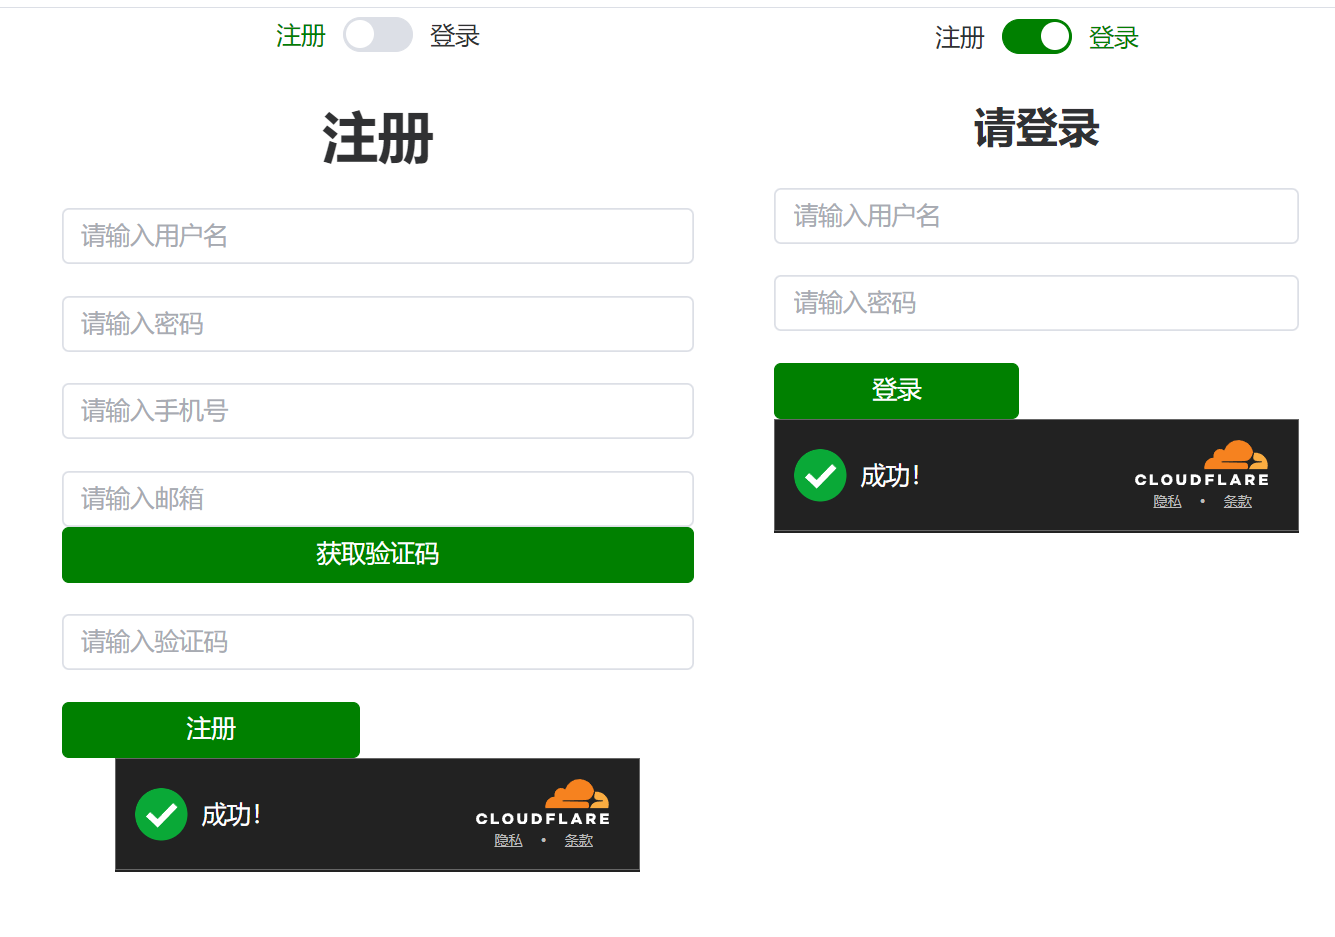
\includegraphics[width=0.8\textwidth]{assets/image-20240429120546182.png}

	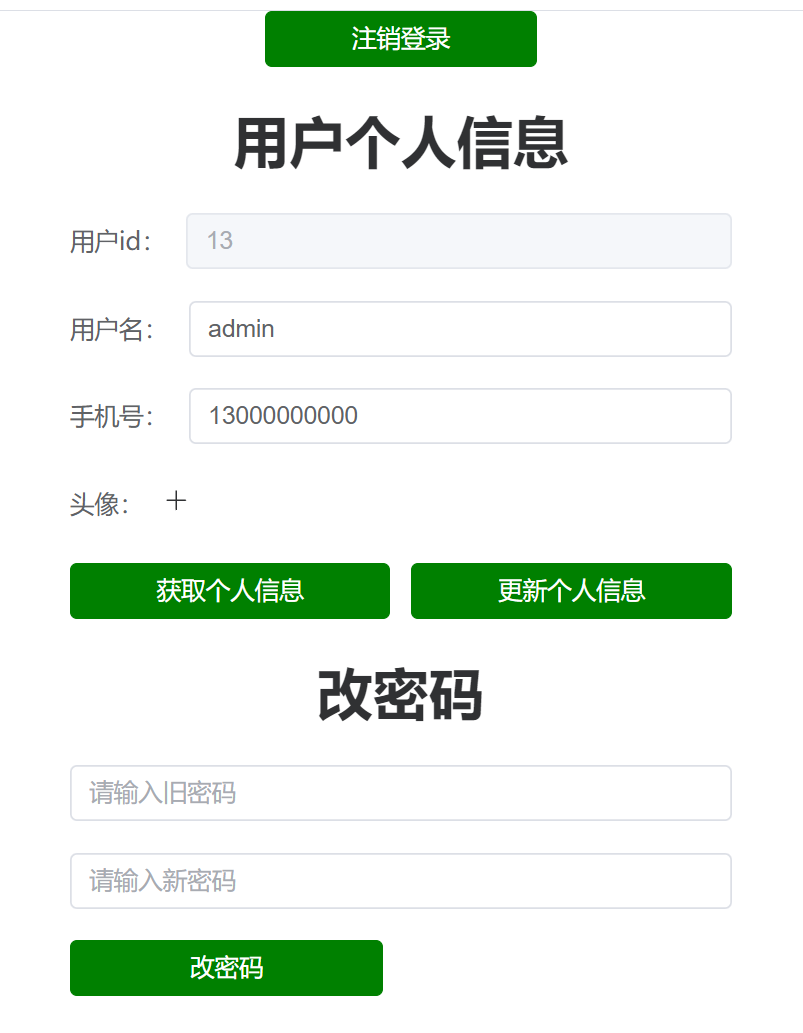
\includegraphics[width=0.8\textwidth]{assets/image-20240429120637515.png}

\end{frame}


\begin{frame}
	\frametitle{群组页面}

	有查看群组列表,创建群组和查看我的群组功能。

	创建群组将会向网站管理员发送申请,管理员审批通过即成功创建群组。

	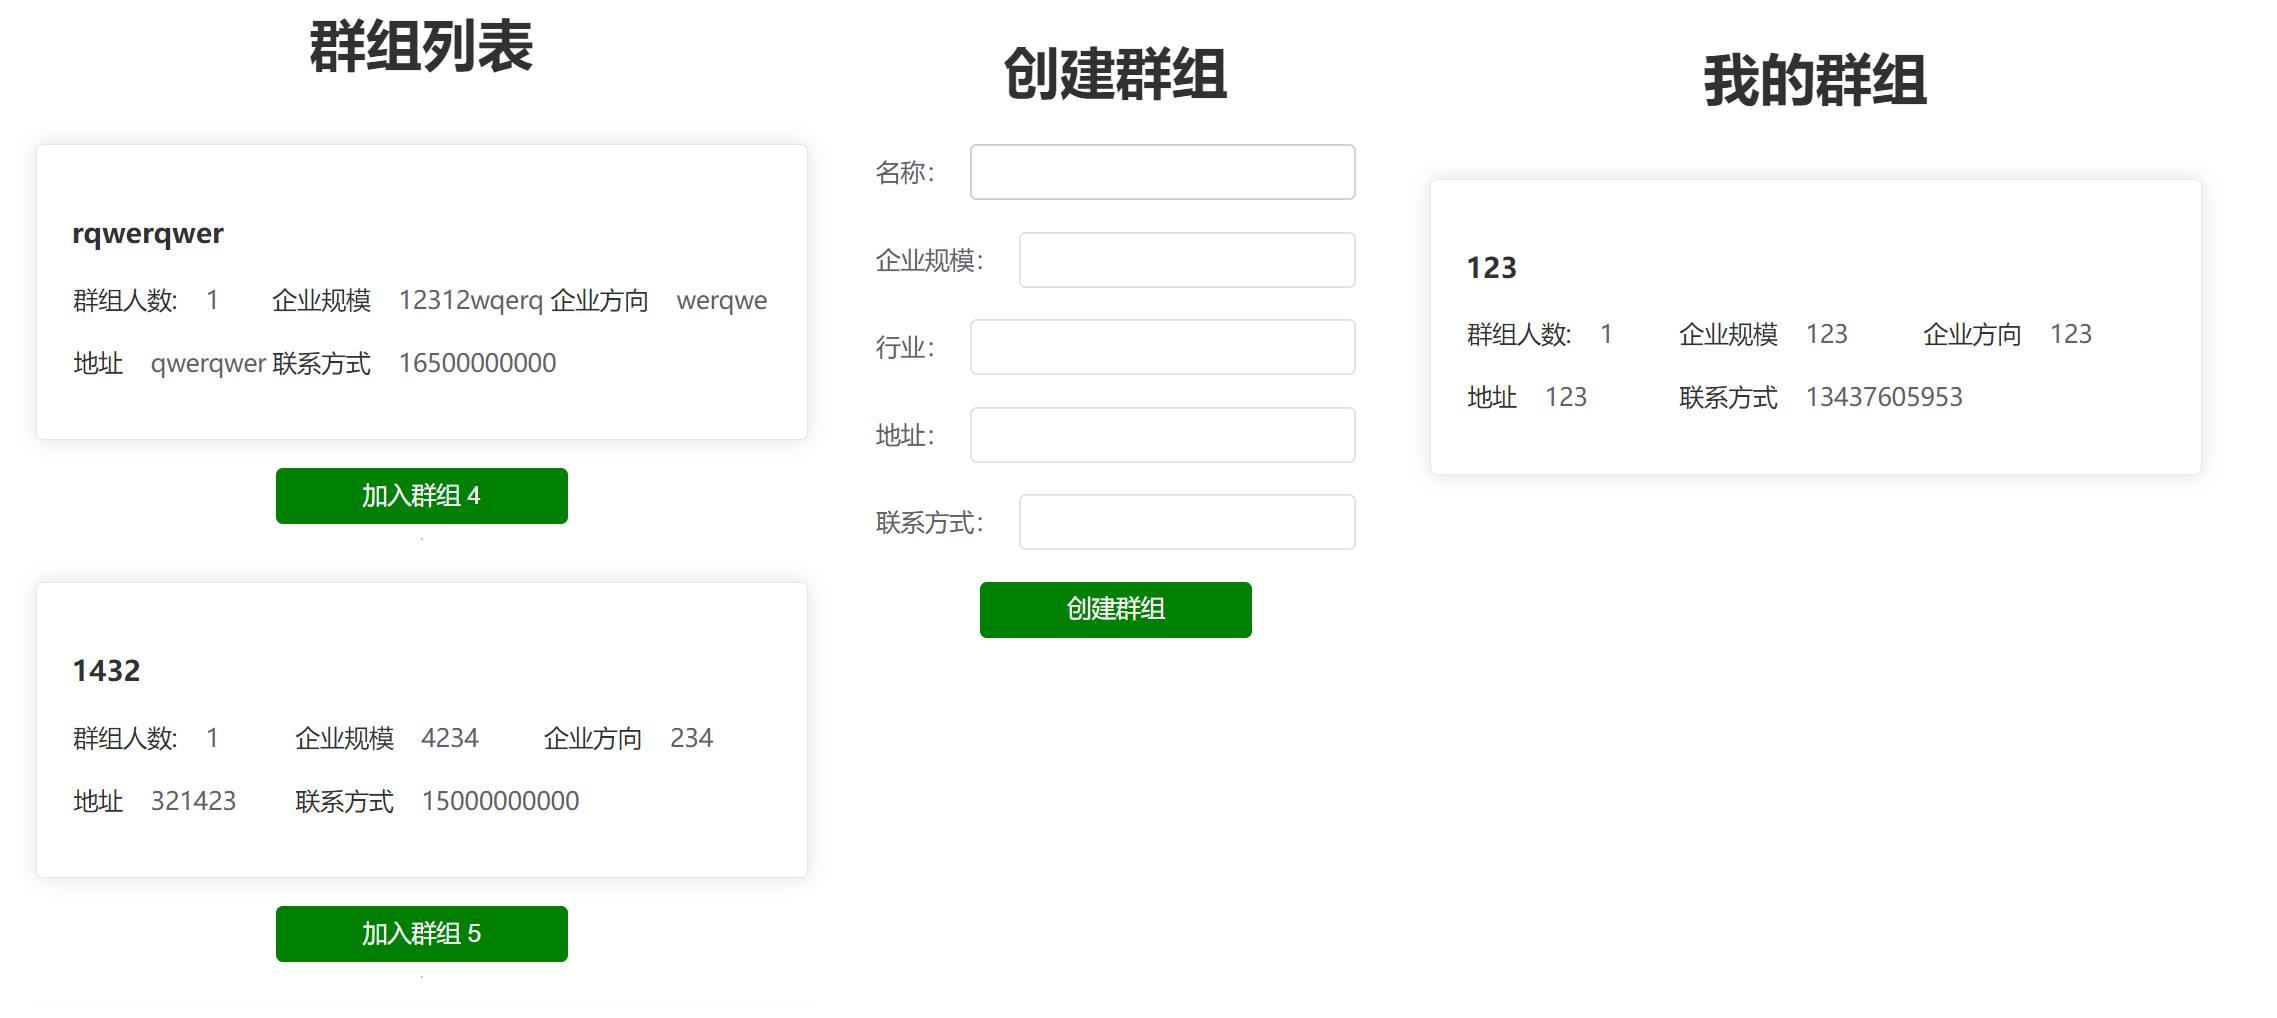
\includegraphics[width=0.8\textwidth]{assets/image-20240429120922179.png}

\end{frame}


\begin{frame}
	\frametitle{群组页面}

	\begin{minipage}{0.4\linewidth}
		网站管理员会比普通用户多出来可以封禁群组和解封群组的功能,被封禁的群组无法做任何操作,同时群组钱包会被冻结,无法进行交易,只能由群组管理员向网站管理员申请解封。
	\end{minipage}\hspace{0.3cm}
	\begin{minipage}{0.45\linewidth}
		\begin{figure}[h]
			\centering
			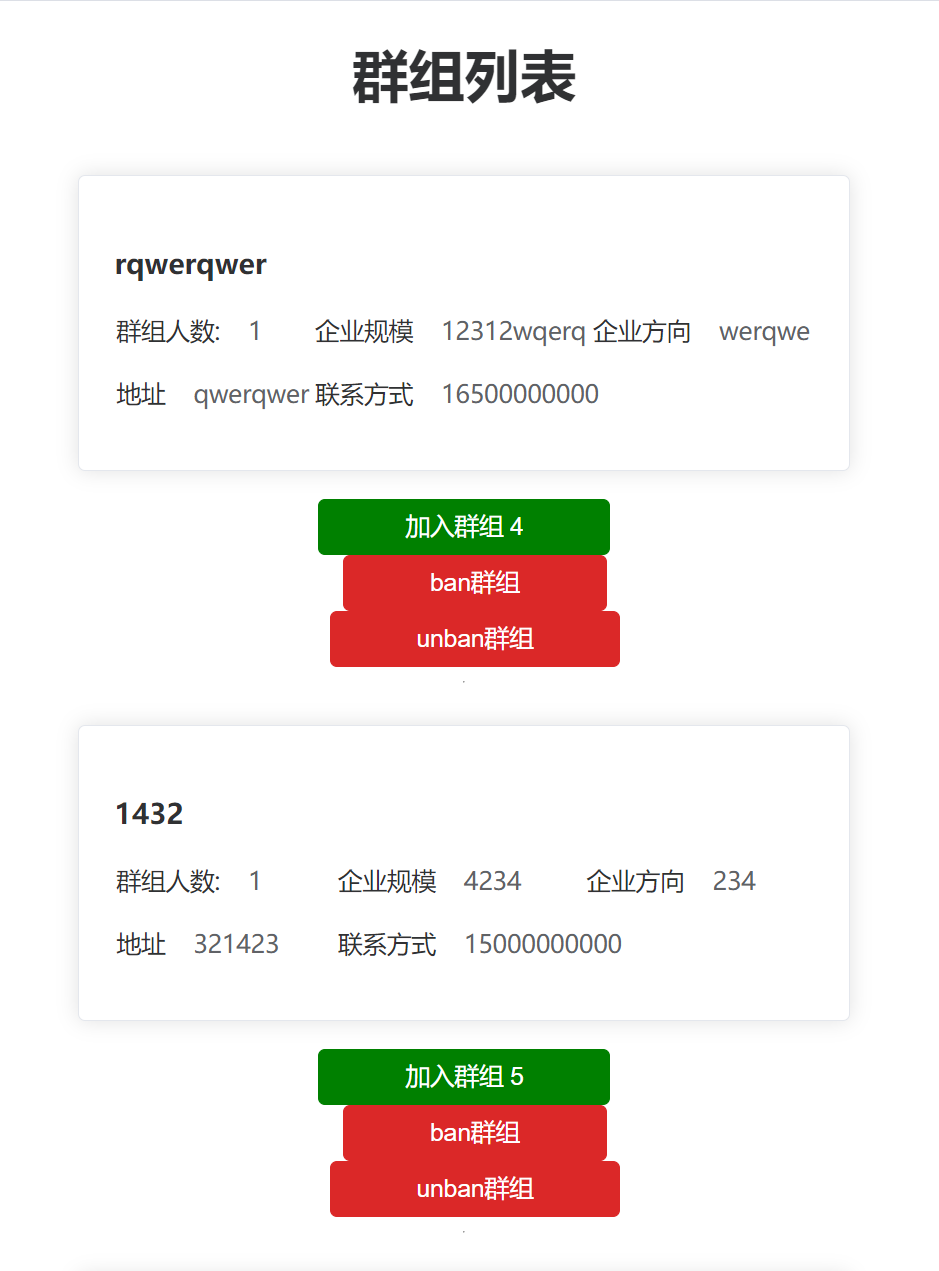
\includegraphics[height=\textheight]{assets/image-20240429131202427.png}
		\end{figure}
	\end{minipage}%\hspace{0.1cm}

\end{frame}


\begin{frame}
	\frametitle{群组详细页面}


	\begin{minipage}{0.4\linewidth}
		用户可以查看自己的群组的详细信息
	\end{minipage}\hspace{0.3cm}
	\begin{minipage}{0.45\linewidth}
		\begin{figure}[h]
			\centering
			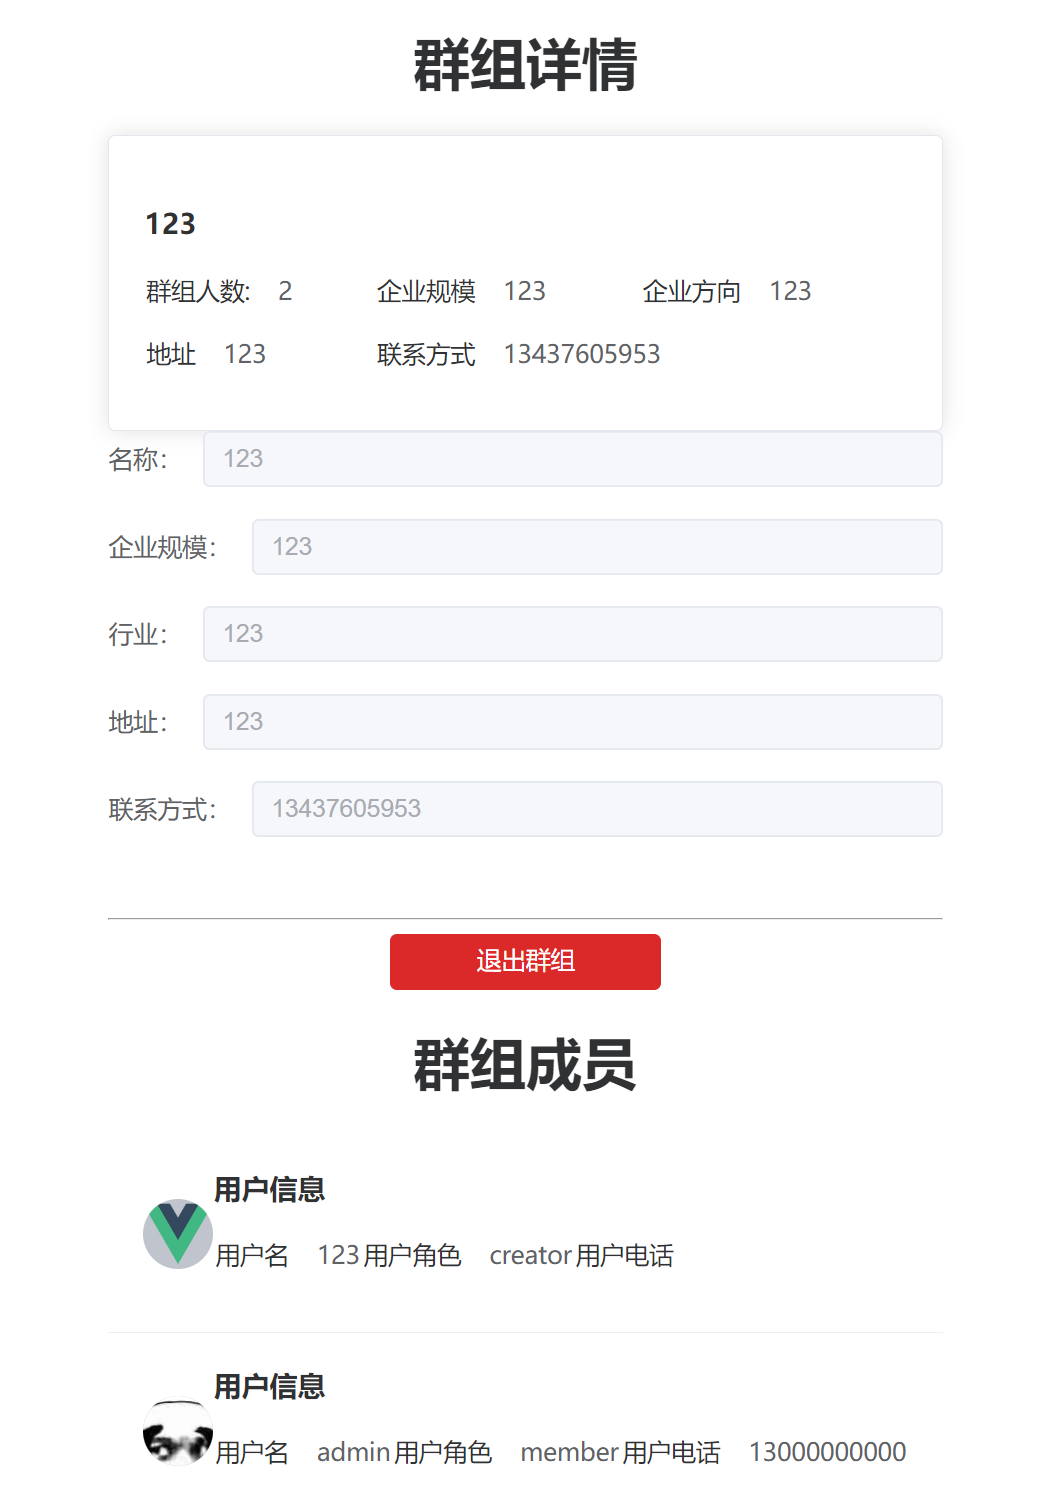
\includegraphics[height=\textheight]{assets/image-20240429122236442.png}

		\end{figure}
	\end{minipage}%\hspace{0.1cm}

\end{frame}



\begin{frame}
	\frametitle{群组详细页面}
	\begin{minipage}{0.4\linewidth}
		群组管理员会比普通的群组成员多出管理方面的功能
	\end{minipage}
	%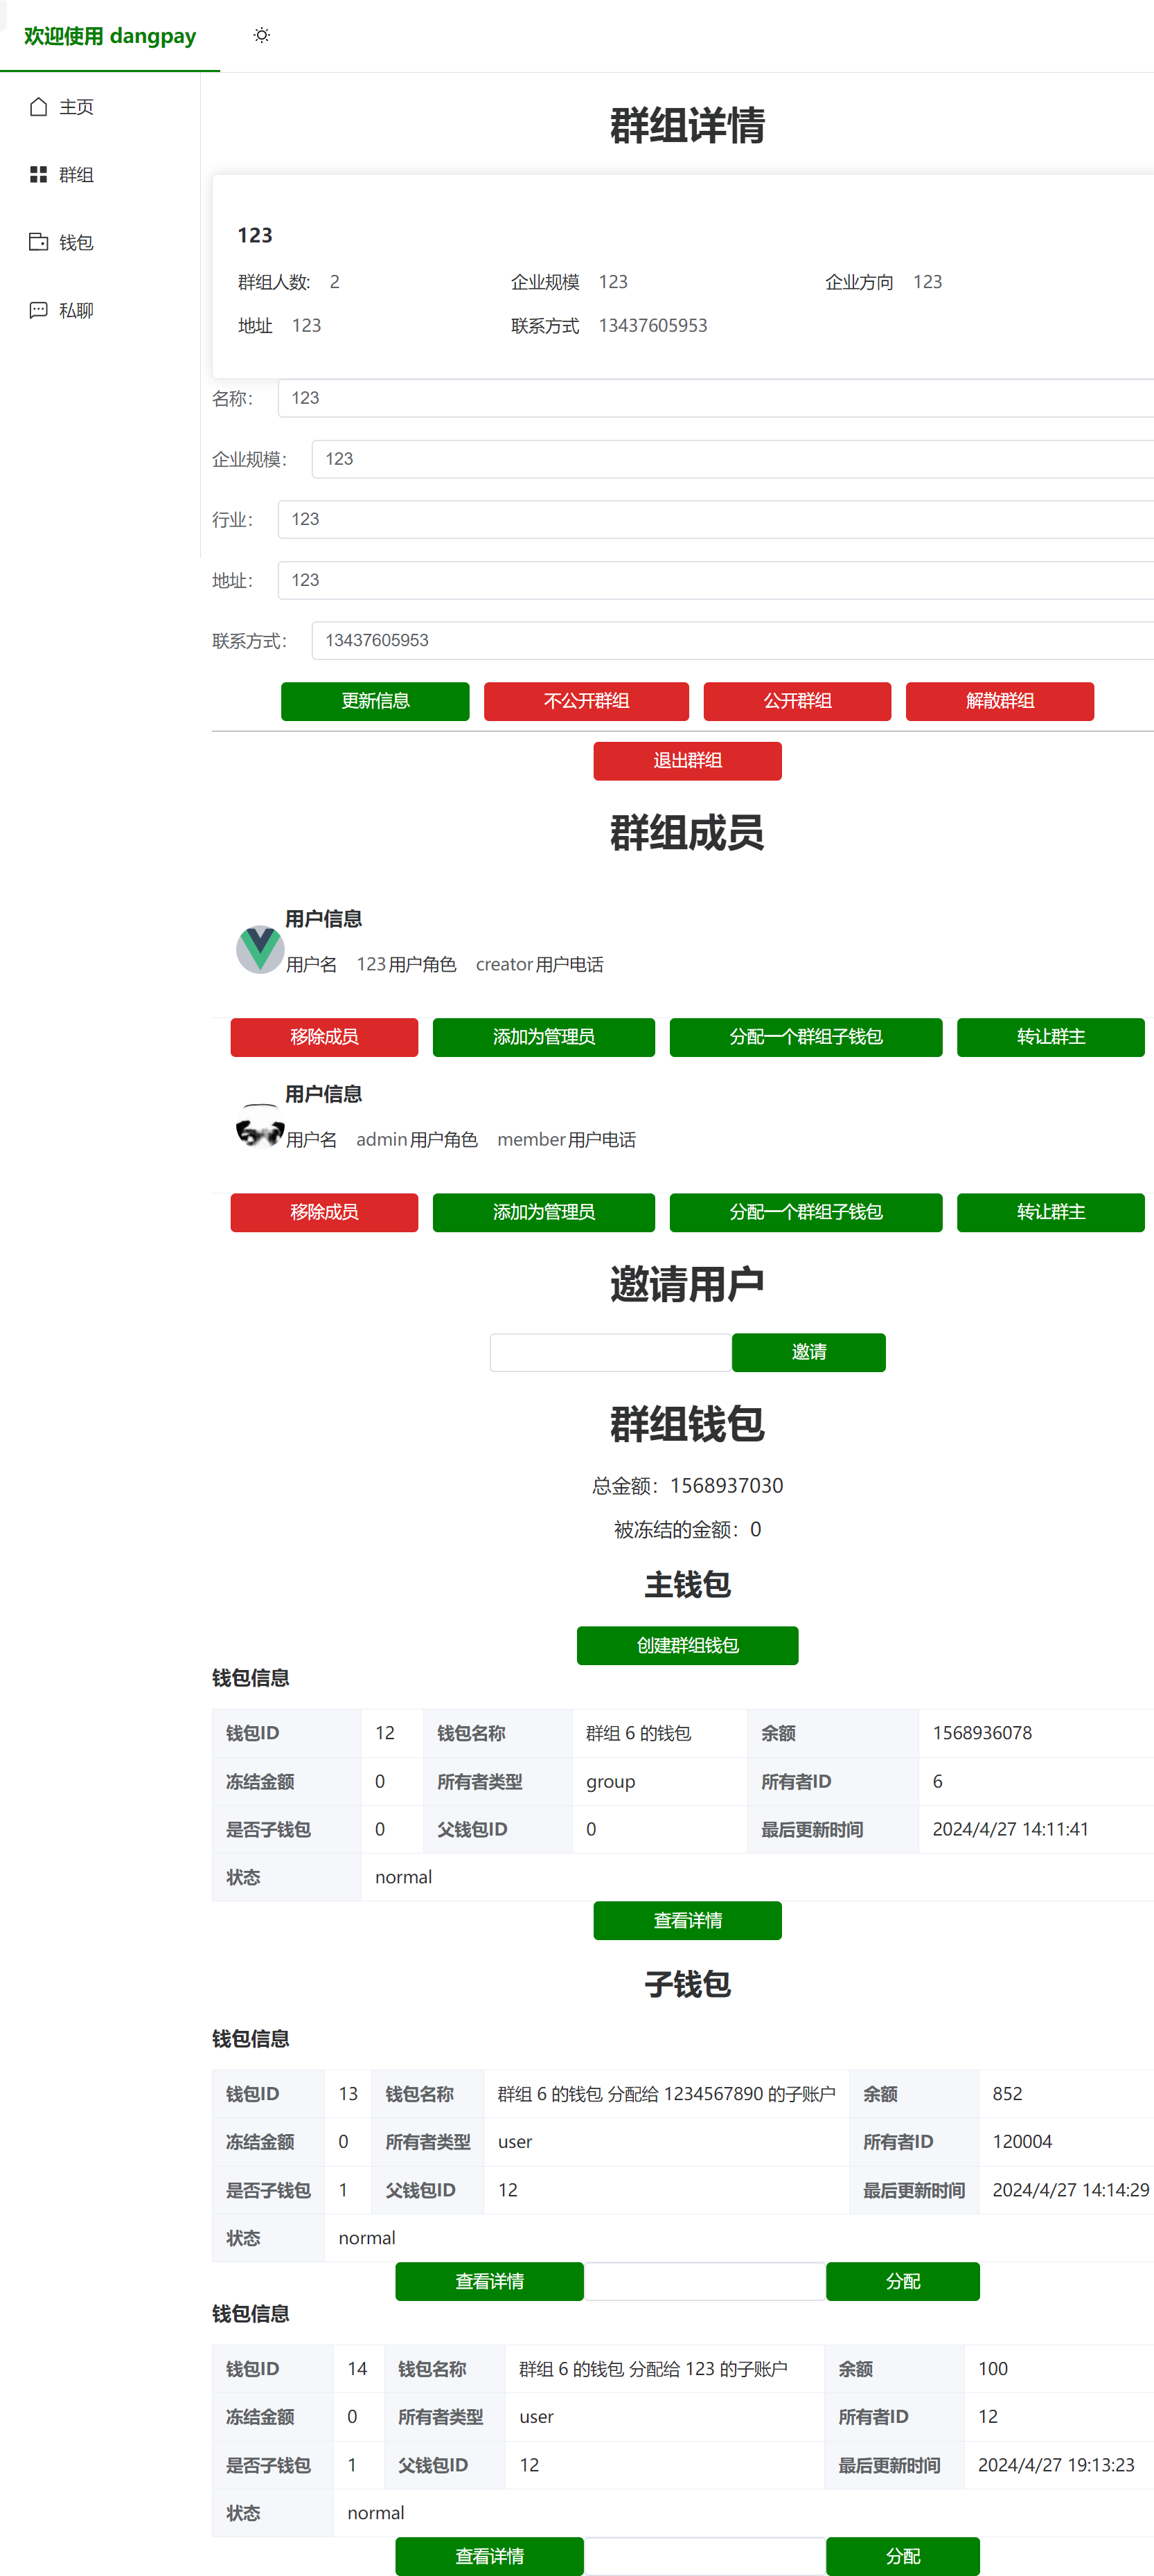
\includegraphics[width=0.4\textwidth]{assets/dangpay.99.suyiiyii.top_ (1)_1.png}
	\hspace{0.3cm}
	\begin{figure}
		\centering
		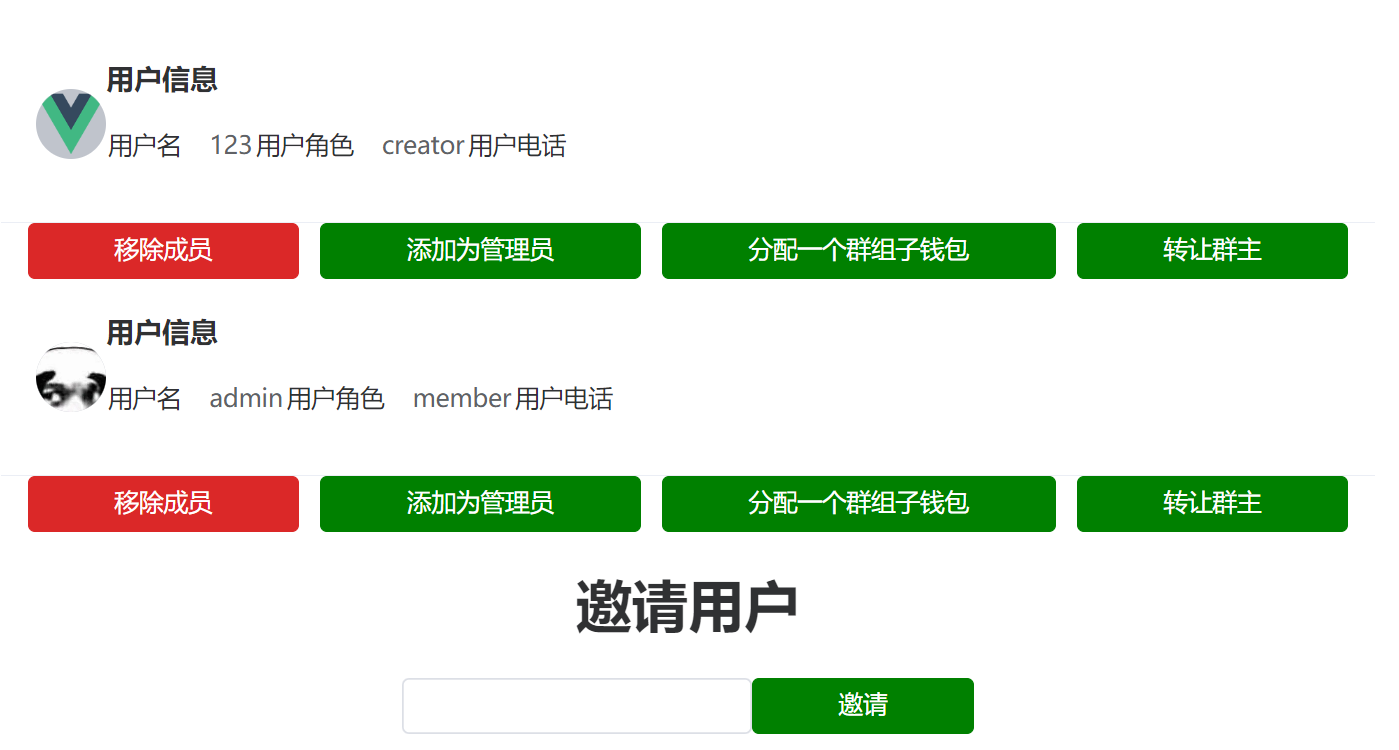
\includegraphics[width=0.7\linewidth]{assets/screenshot001}
		\label{fig:screenshot001}
	\end{figure}


\end{frame}


\begin{frame}
	\frametitle{钱包页面}
	\begin{center}
		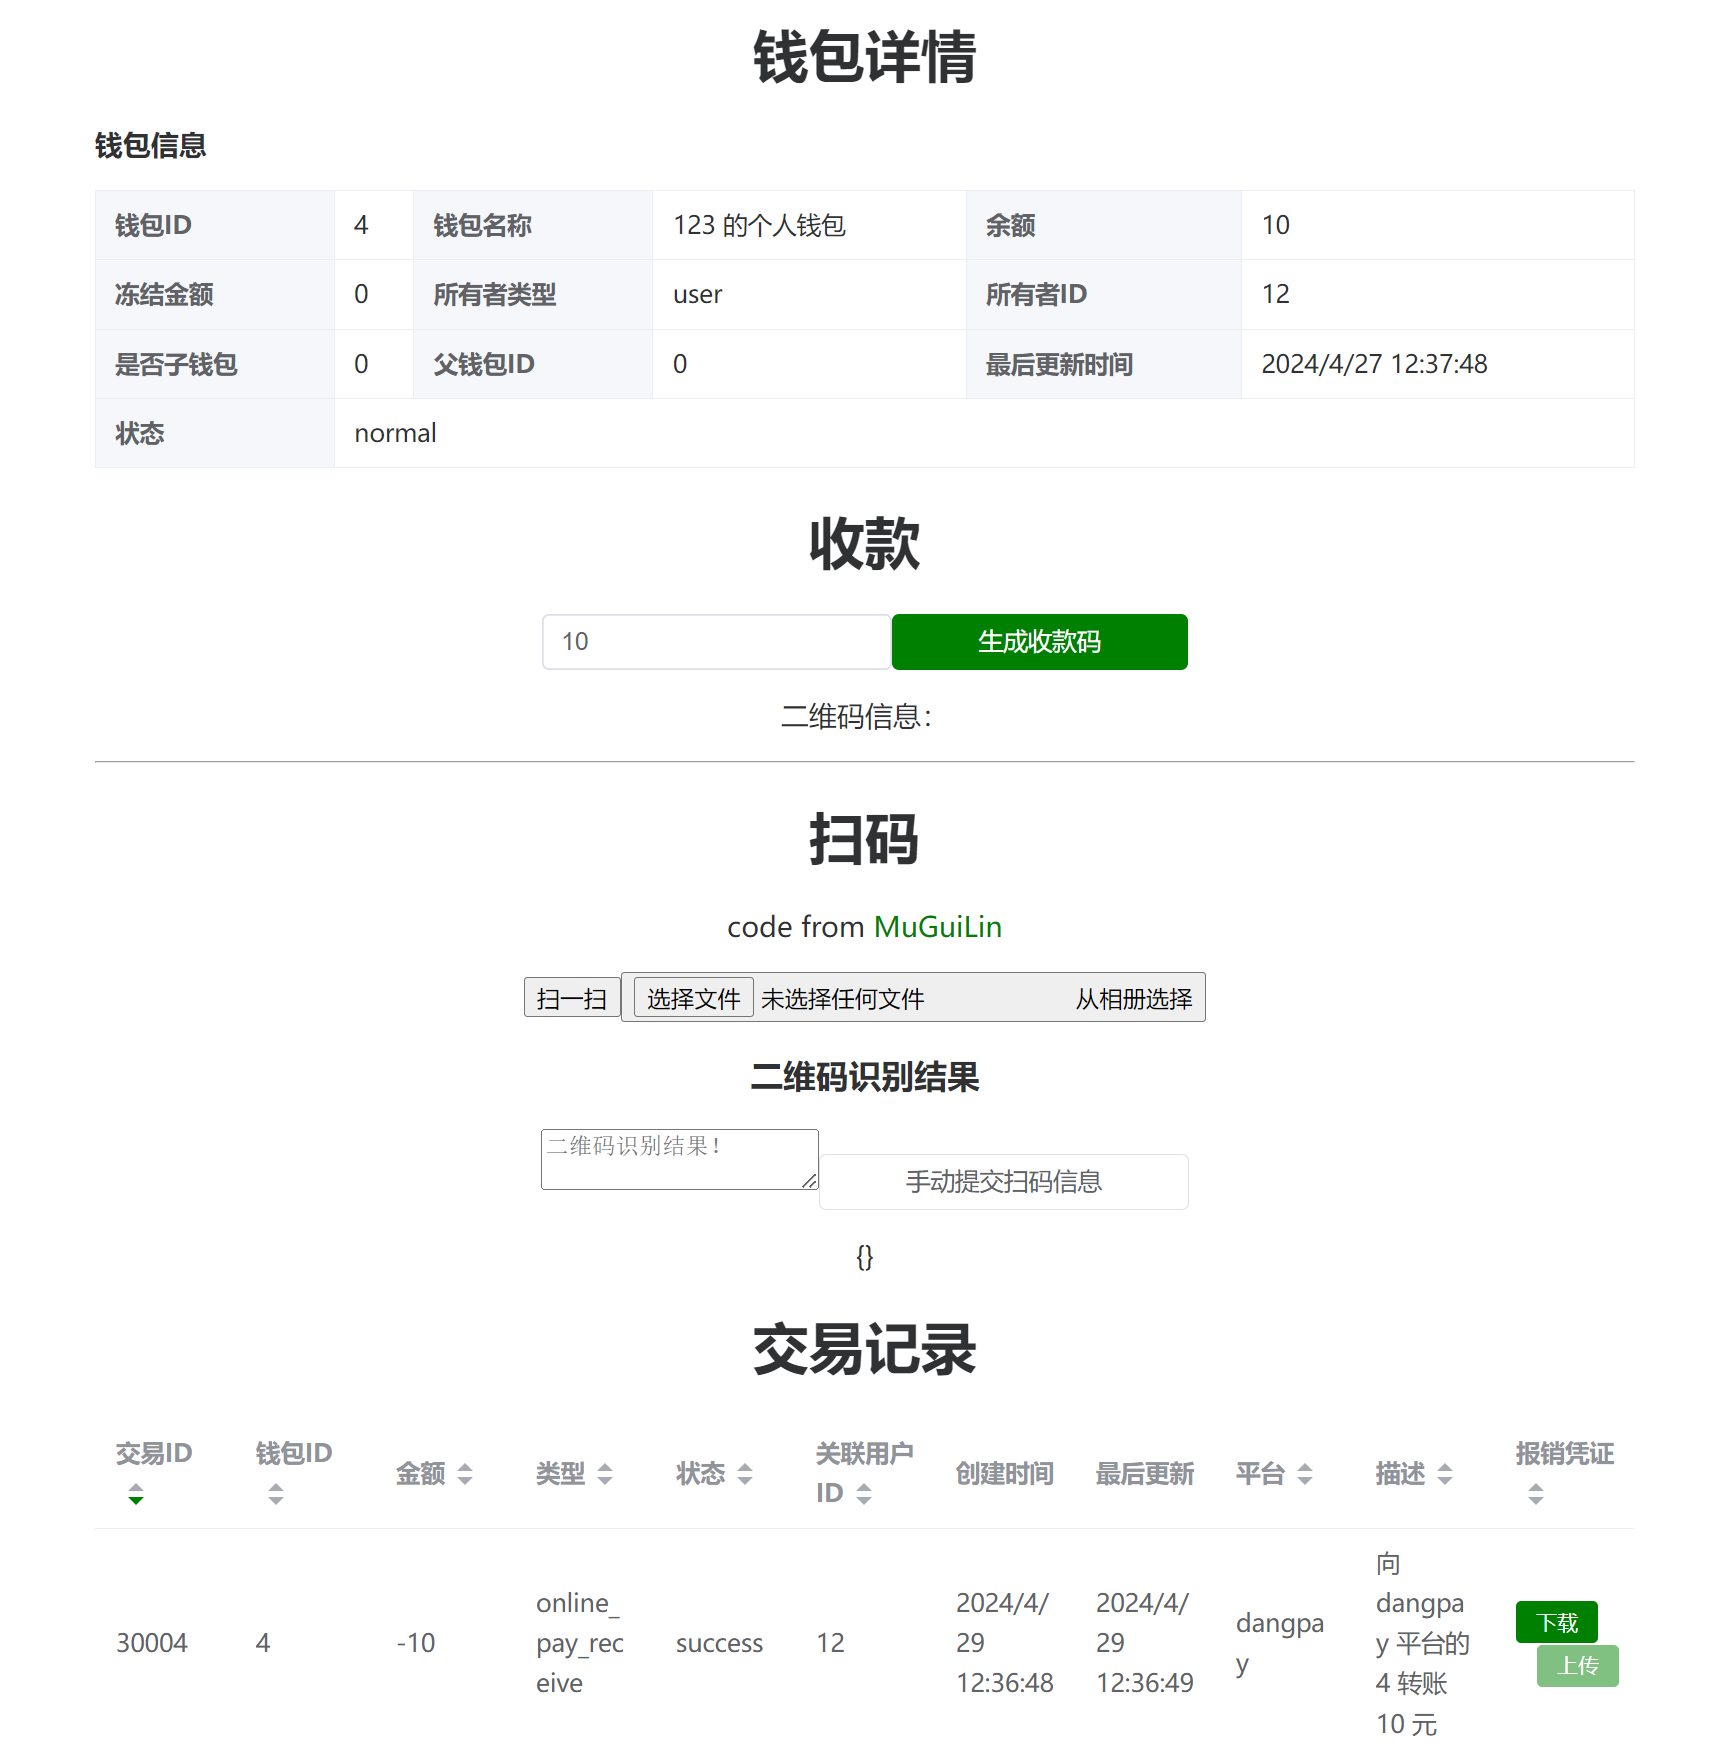
\includegraphics[width=\linewidth]{assets/screenshot002}
	\end{center}

\end{frame}



\begin{frame}
	\frametitle{私聊页面}
	用户可以在这里接收和处理系统通知,和其他用户以及群组内聊天
	\begin{minipage}{0.55\linewidth}
		\begin{figure}[h]
			\centering
			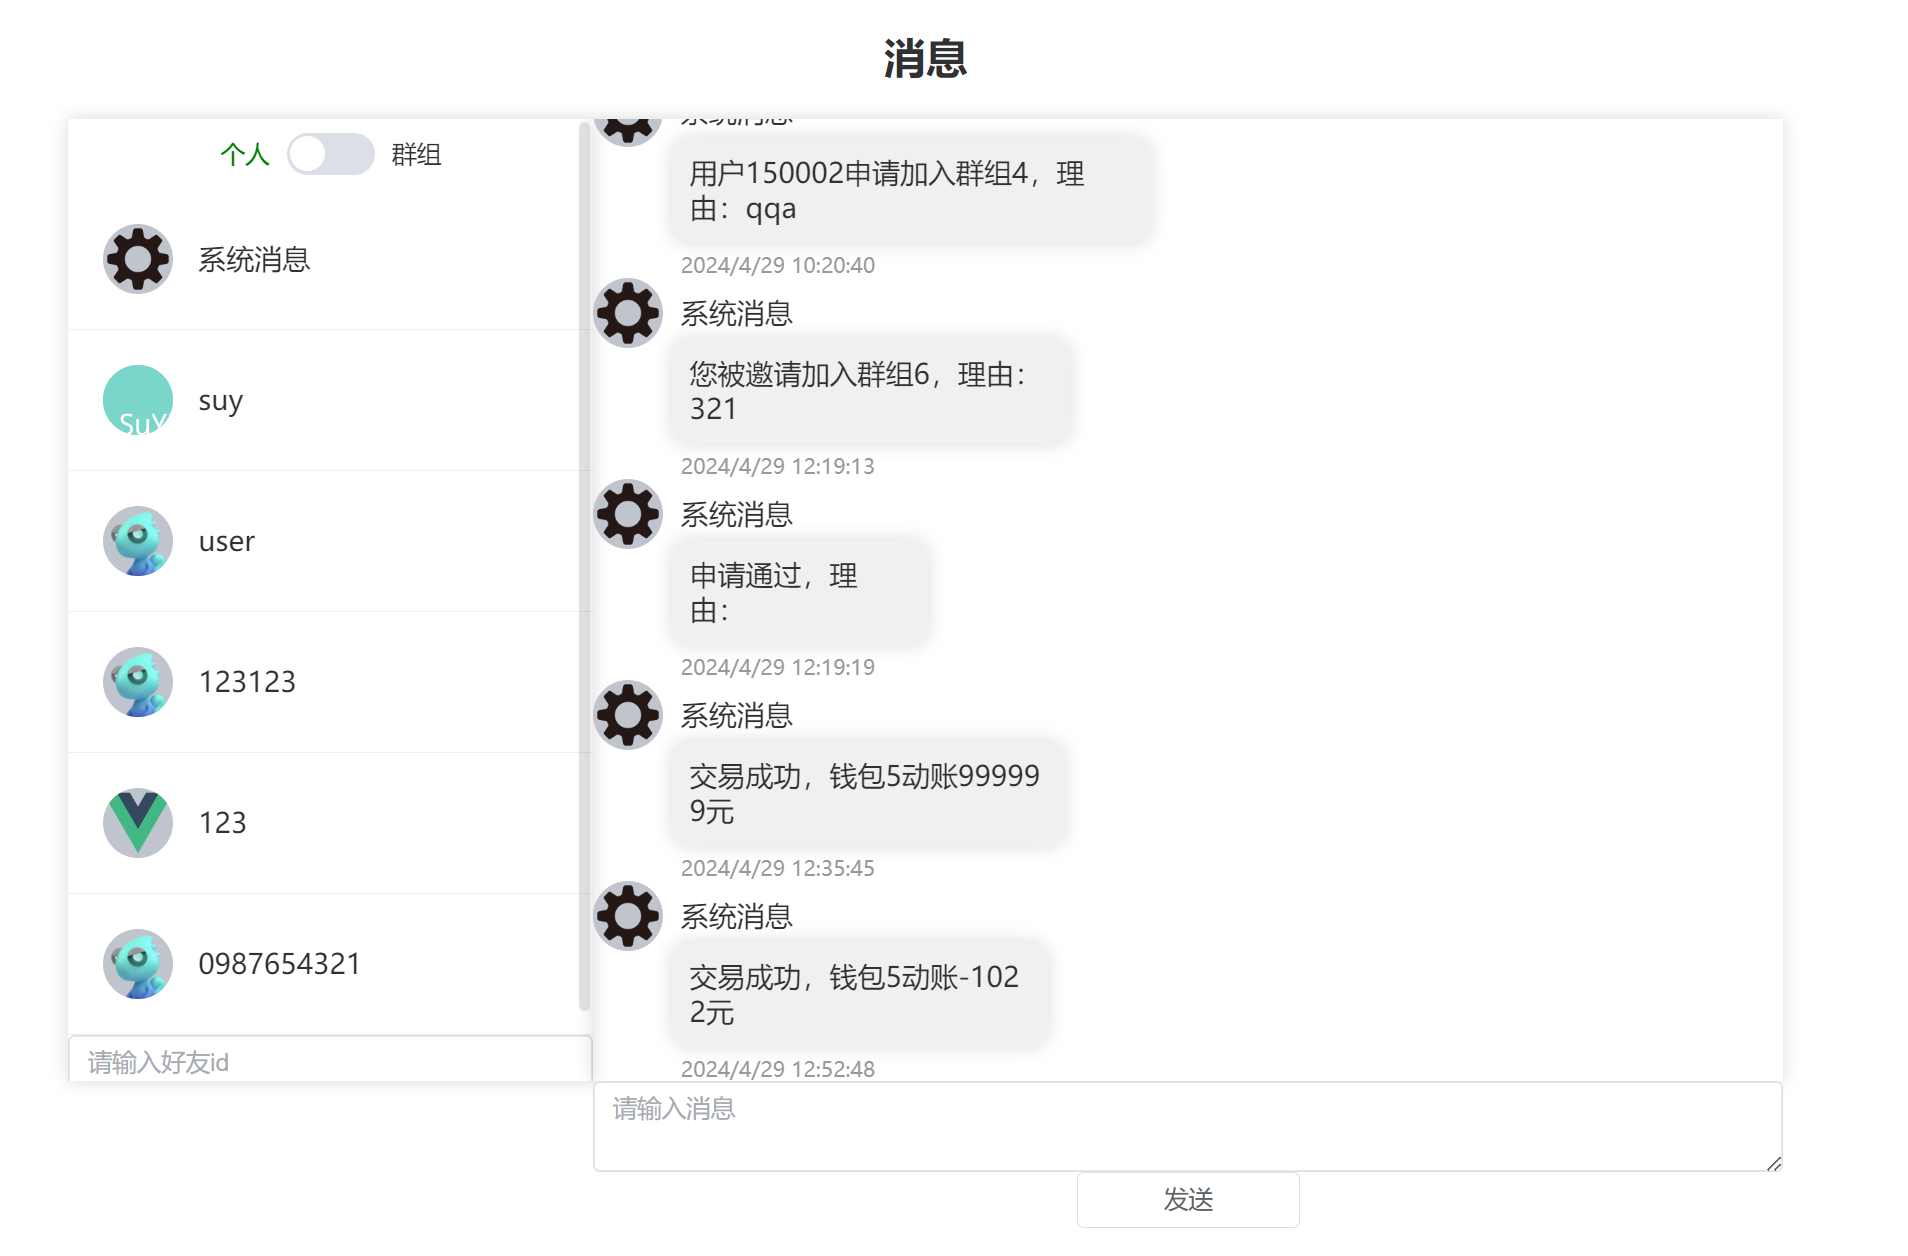
\includegraphics[height=\textheight]{assets/image-20240429125550801.png}

		\end{figure}
	\end{minipage}%\hspace{0.1cm}


\end{frame}


\begin{frame}
	\frametitle{全局交易记录}
	管理员可以在这个页面看到站内的所有交易记录,便于监管。

	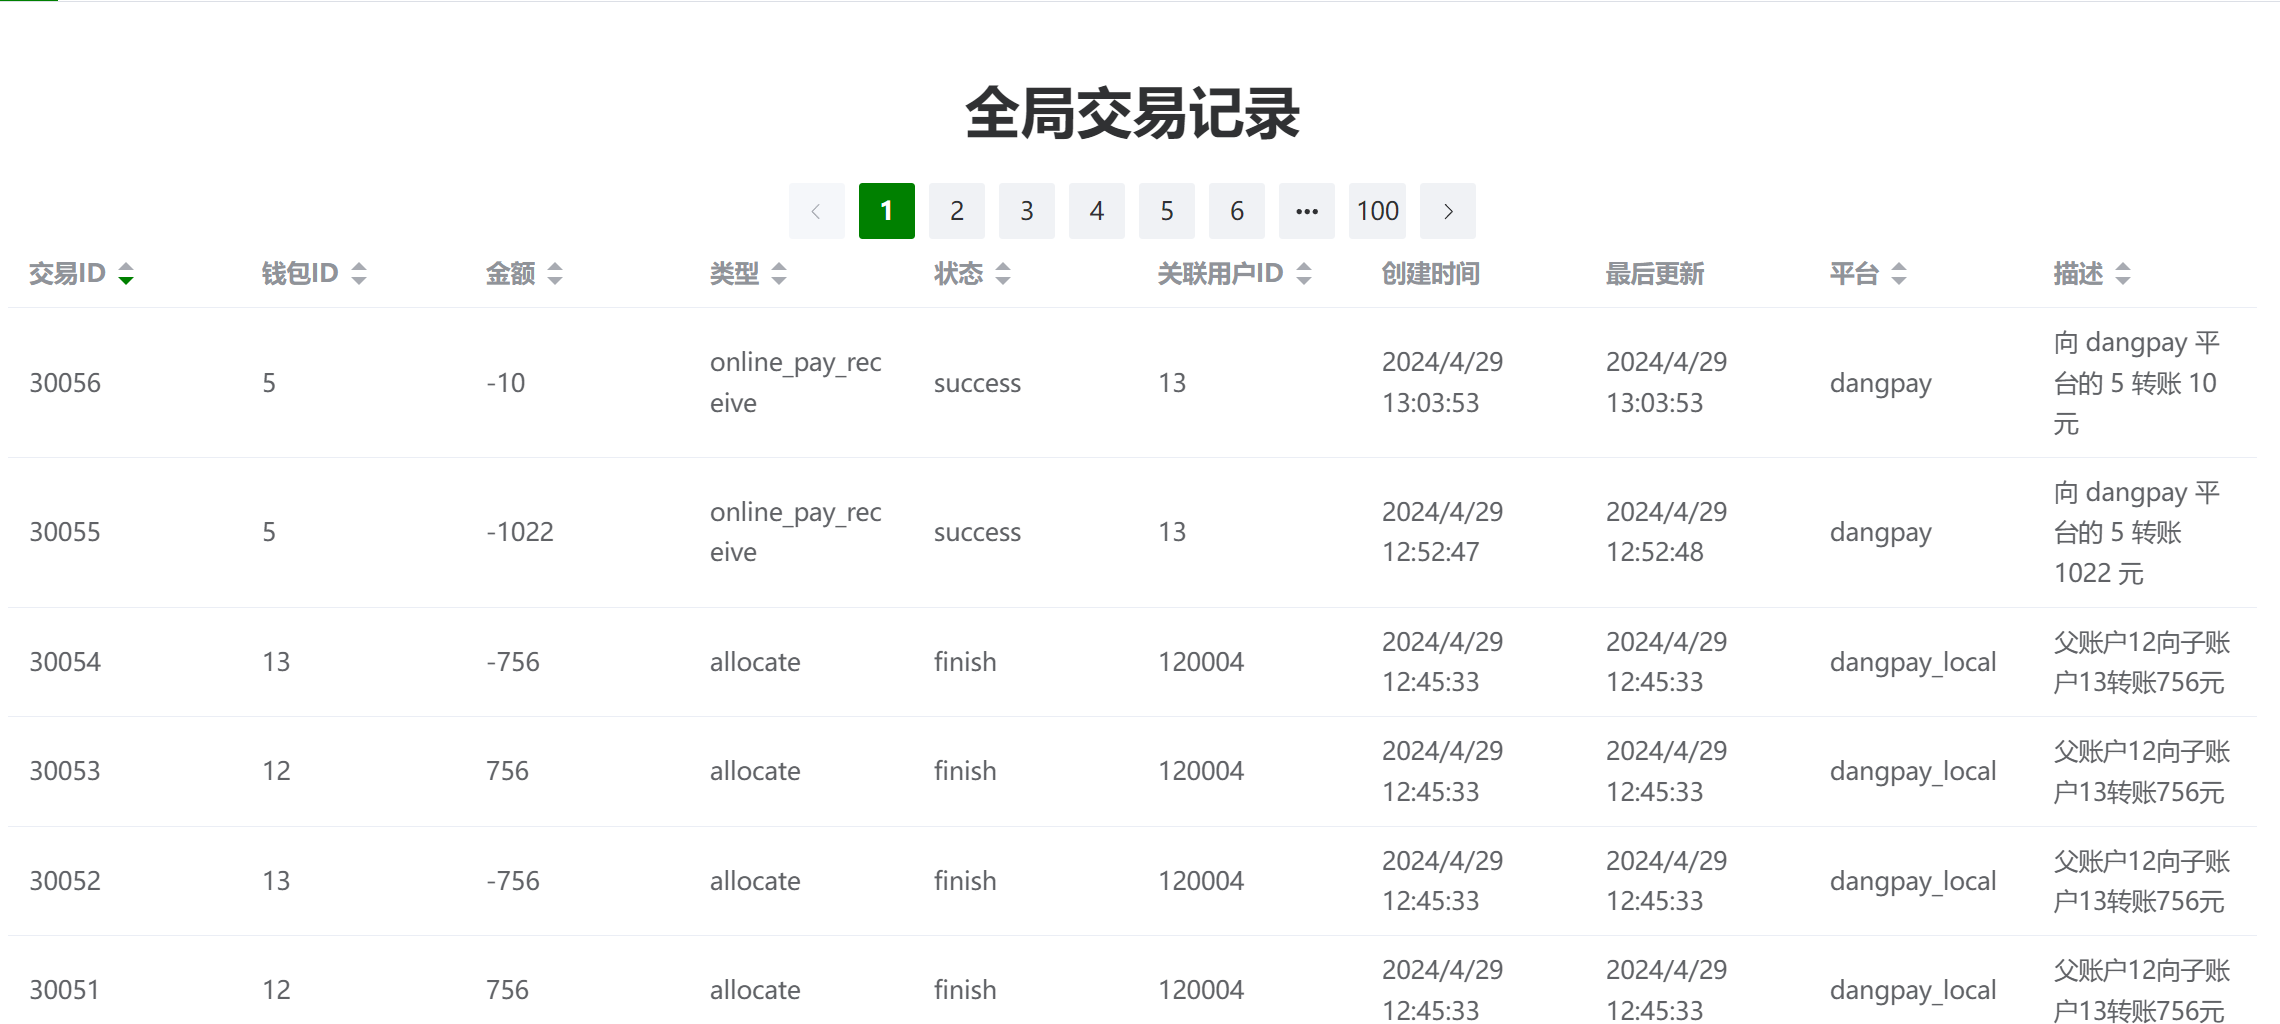
\includegraphics[width=1.2\textwidth]{assets/image-20240429130439225.png}

\end{frame}


\begin{frame}
	\frametitle{审计日志}
	管理员可以查看全站的审计日志,便于查找恶意用户。

	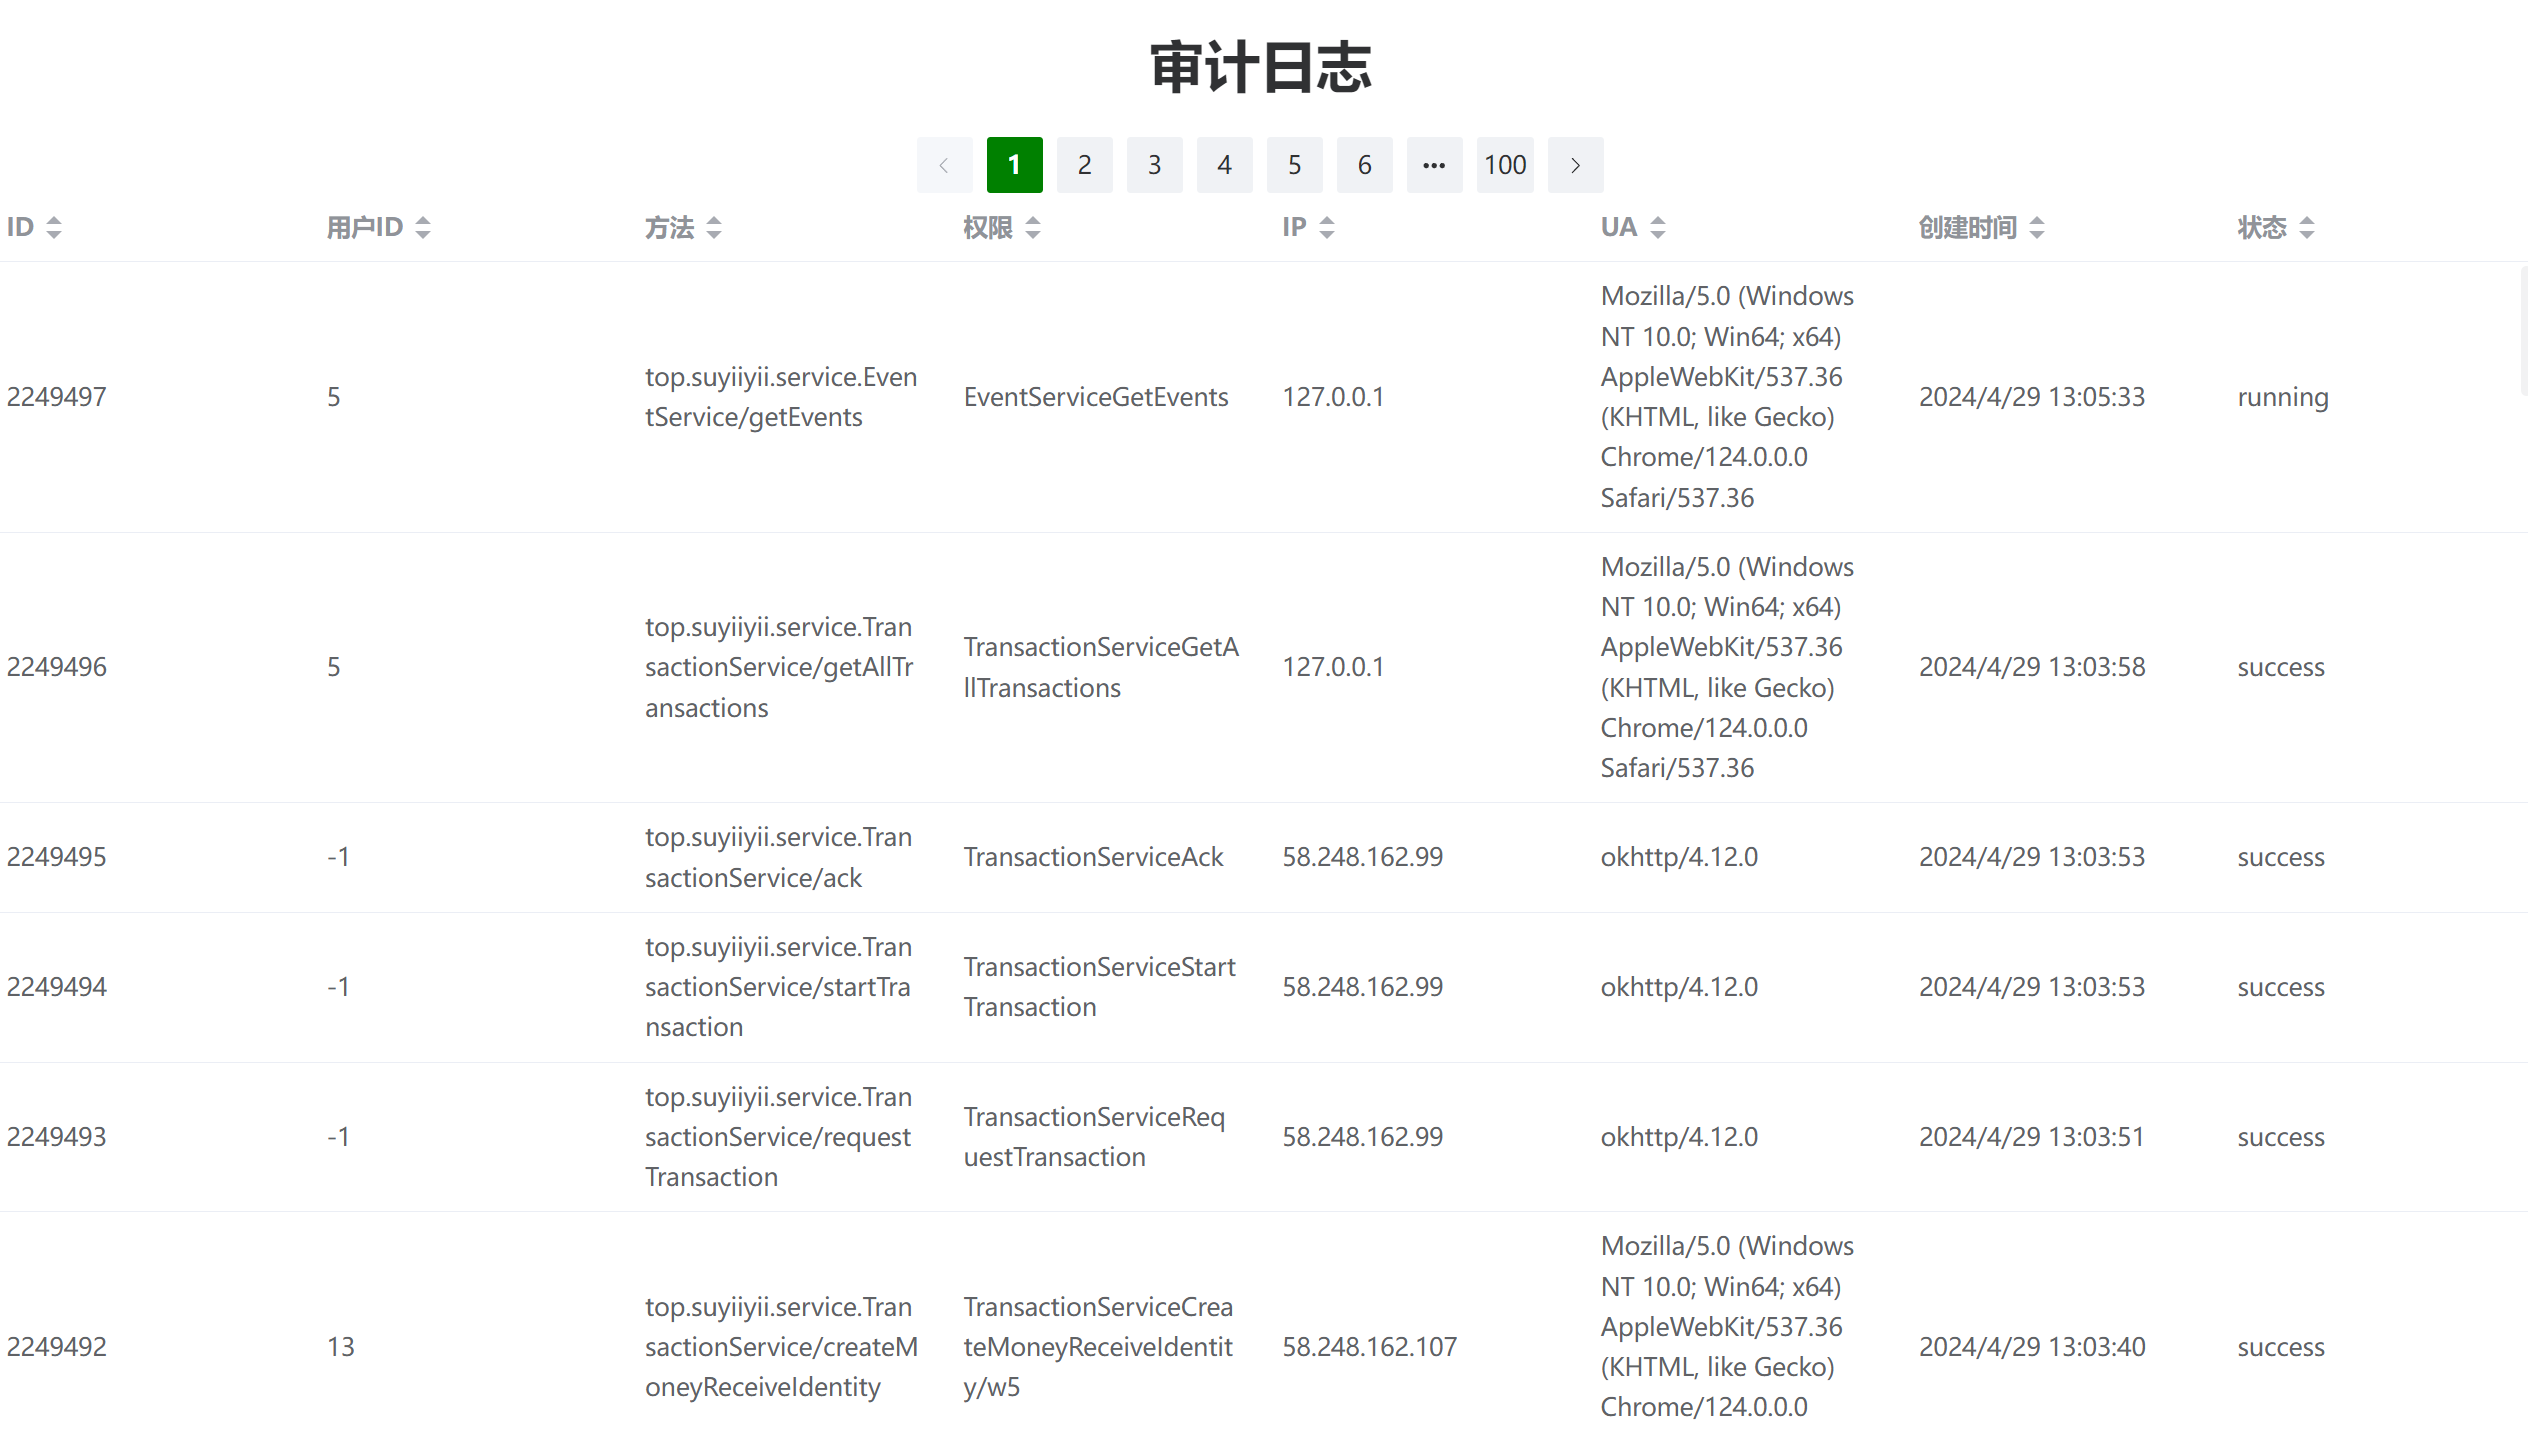
\includegraphics[width=1.2\textwidth]{assets/image-20240429130553723.png}

\end{frame}



\section{设计思路}



\begin{frame}{技术选型}

	%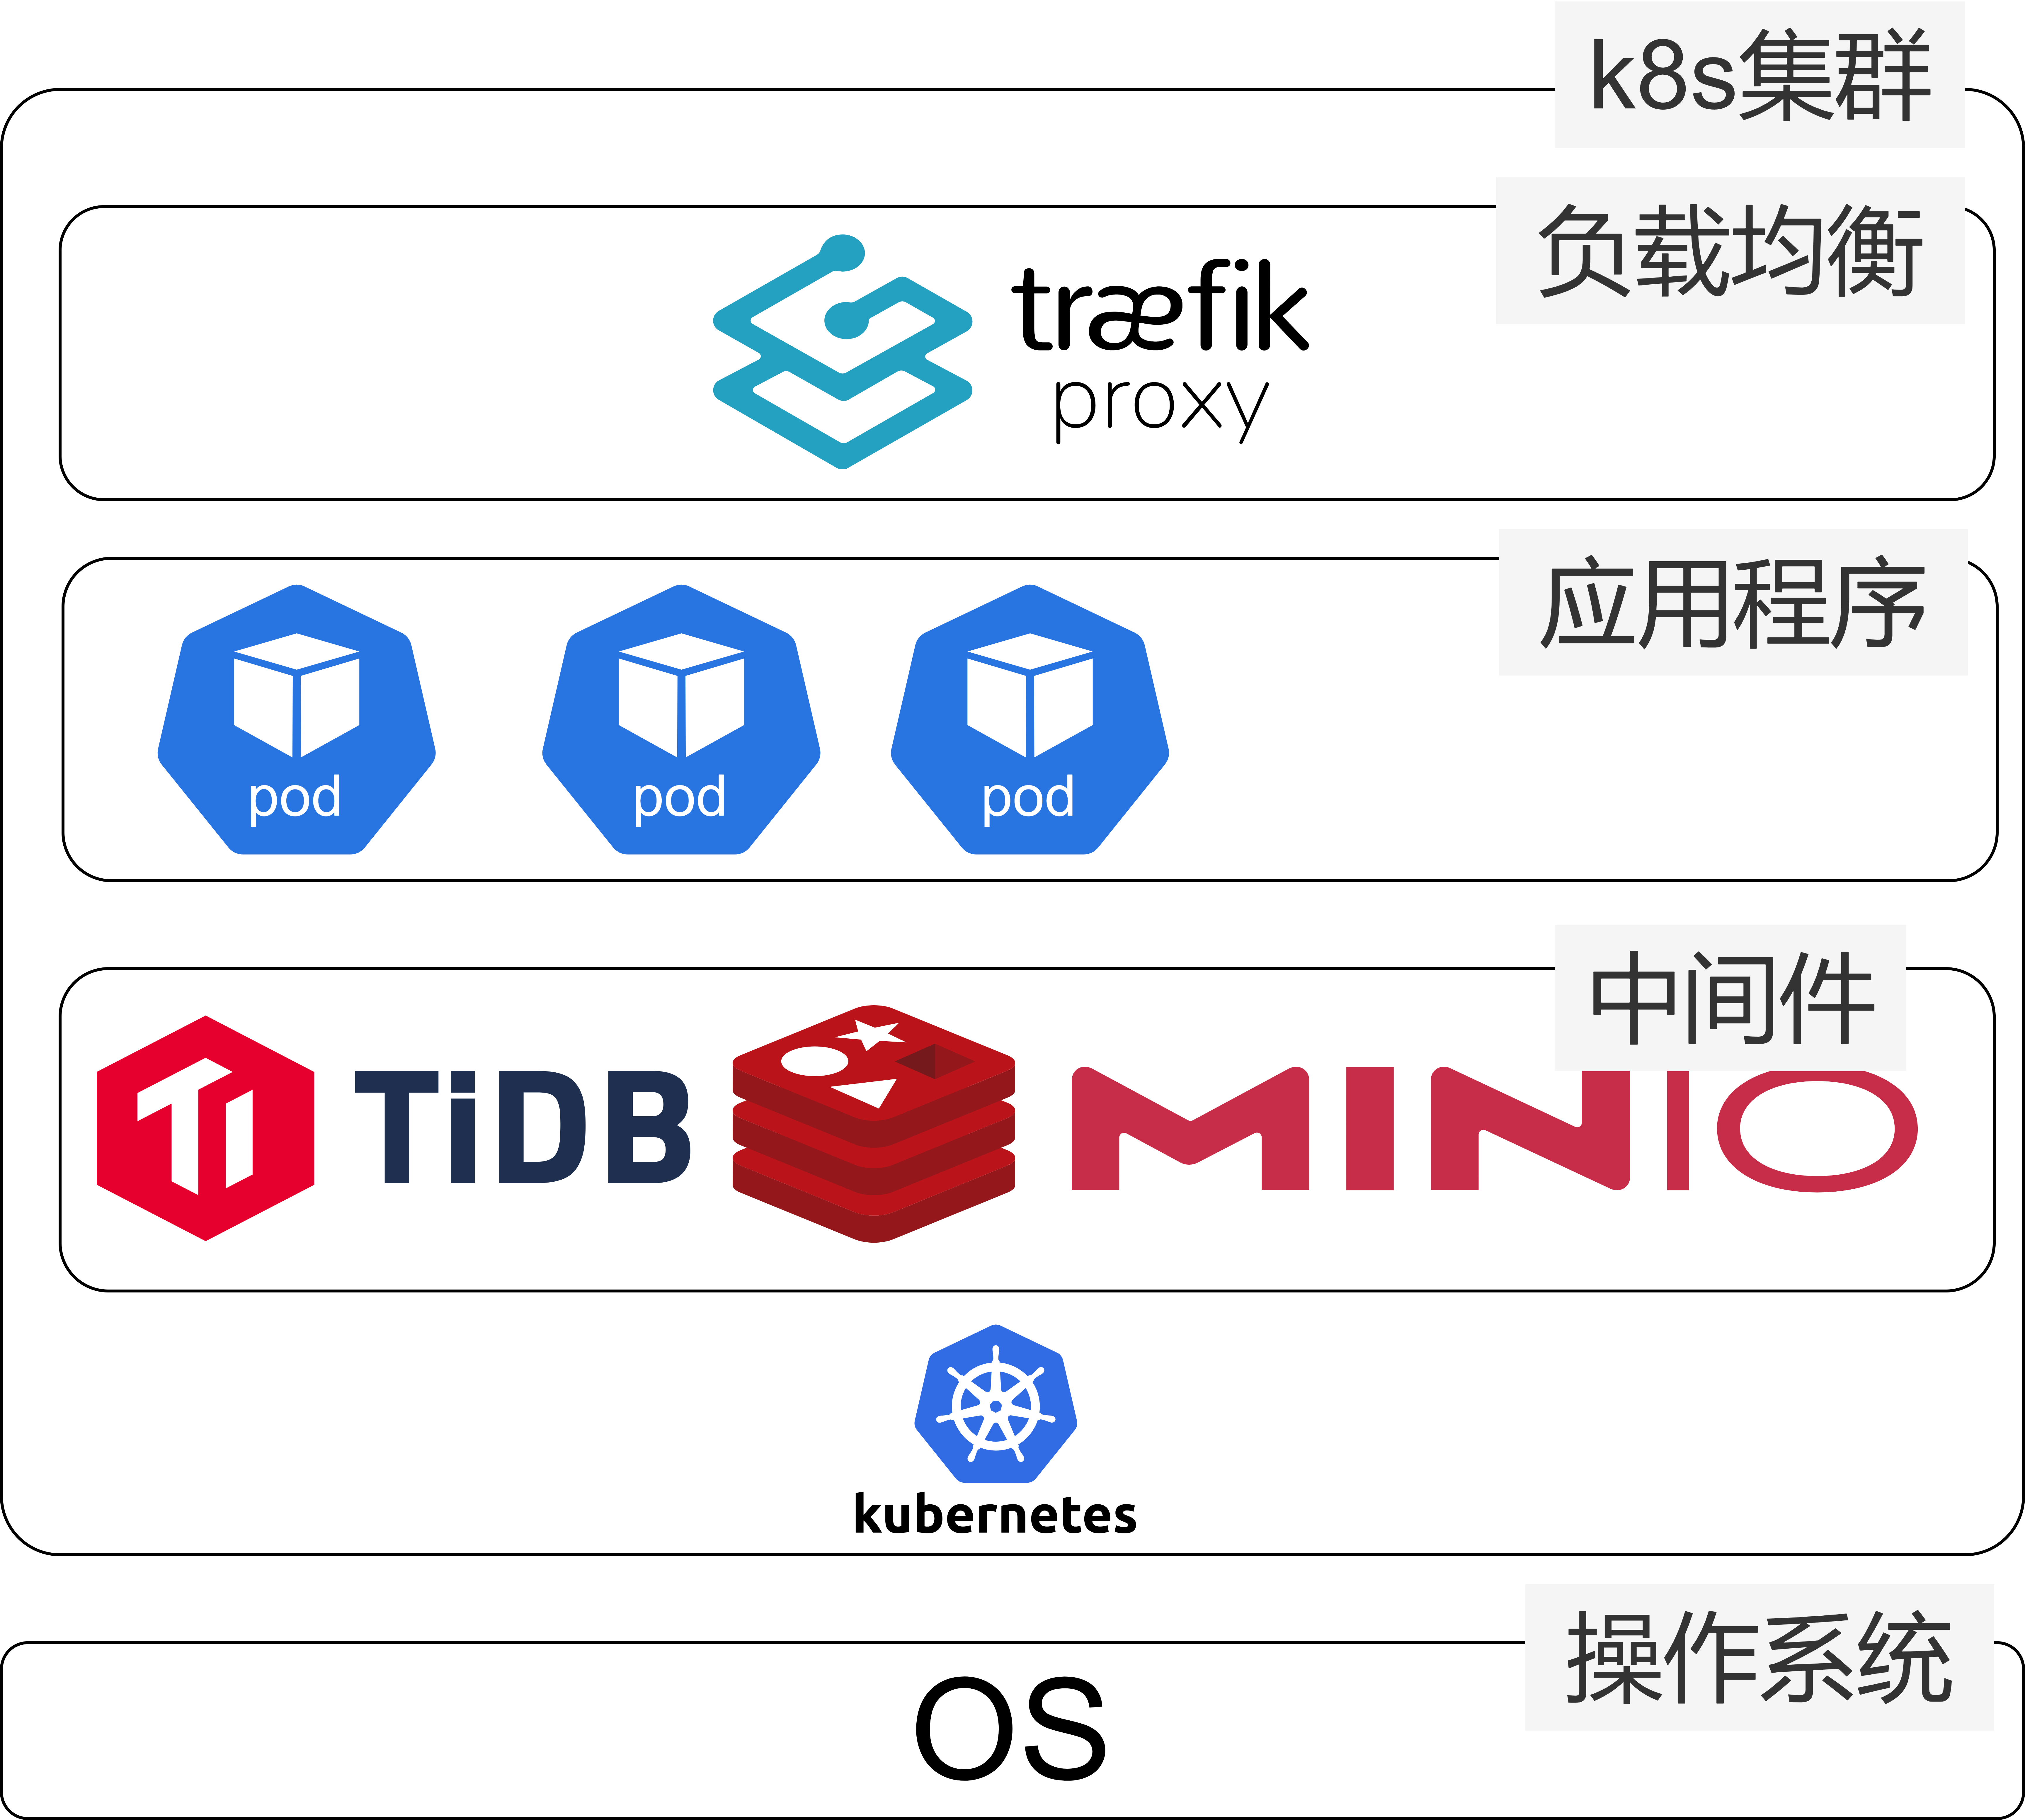
\includegraphics[height=0.8\textheight]{assets/导出 (1).png}
\end{frame}

%------------------------------------------------


\section{项目难点亮点}

\begin{frame}{二维码支付}
	创新性使用二维码的方式支付,方便用户使用
	\begin{block}{对比}
		\begin{minipage}{0.4\linewidth}
			\begin{figure}
				\centering
				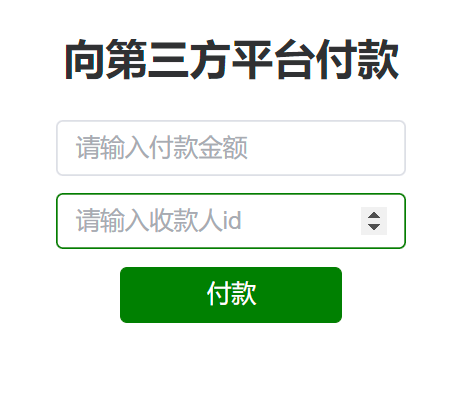
\includegraphics[width=0.9\linewidth]{assets/screenshot005}
				\caption{其他平台的支付方式}
				\label{fig:screenshot005}
			\end{figure}

		\end{minipage}
		\begin{minipage}{0.4\linewidth}
			\begin{figure}
				\centering
				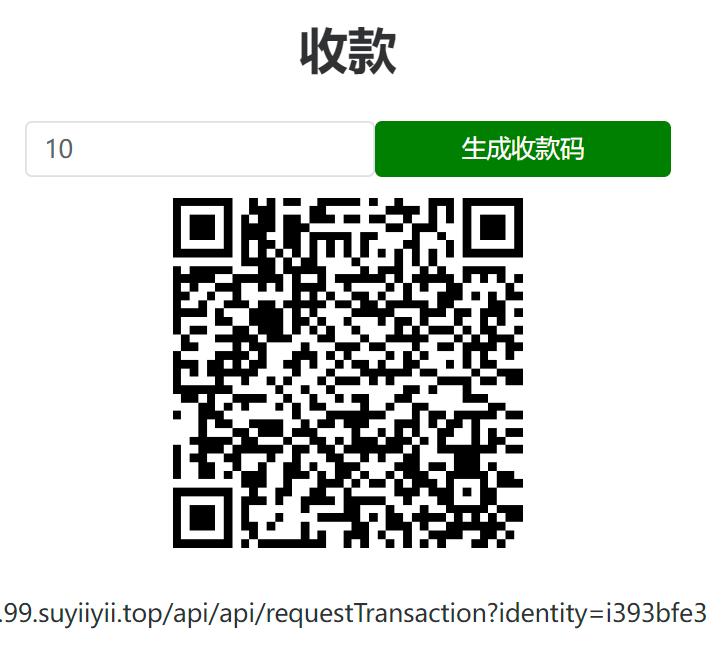
\includegraphics[width=0.9\linewidth]{assets/screenshot006}
				\caption[]{铛铛支付平台支付方式}
				\label{fig:screenshot006}
			\end{figure}

		\end{minipage}

	\end{block}

\end{frame}




\begin{frame}{HTTPS}
	用户请求从浏览器到中转服务器到应用服务器,全程 \texttt{HTTPS/TLS} 加密。
	\begin{block}{对比}
		\begin{minipage}{0.4\linewidth}
			\begin{figure}[h]
				\centering
				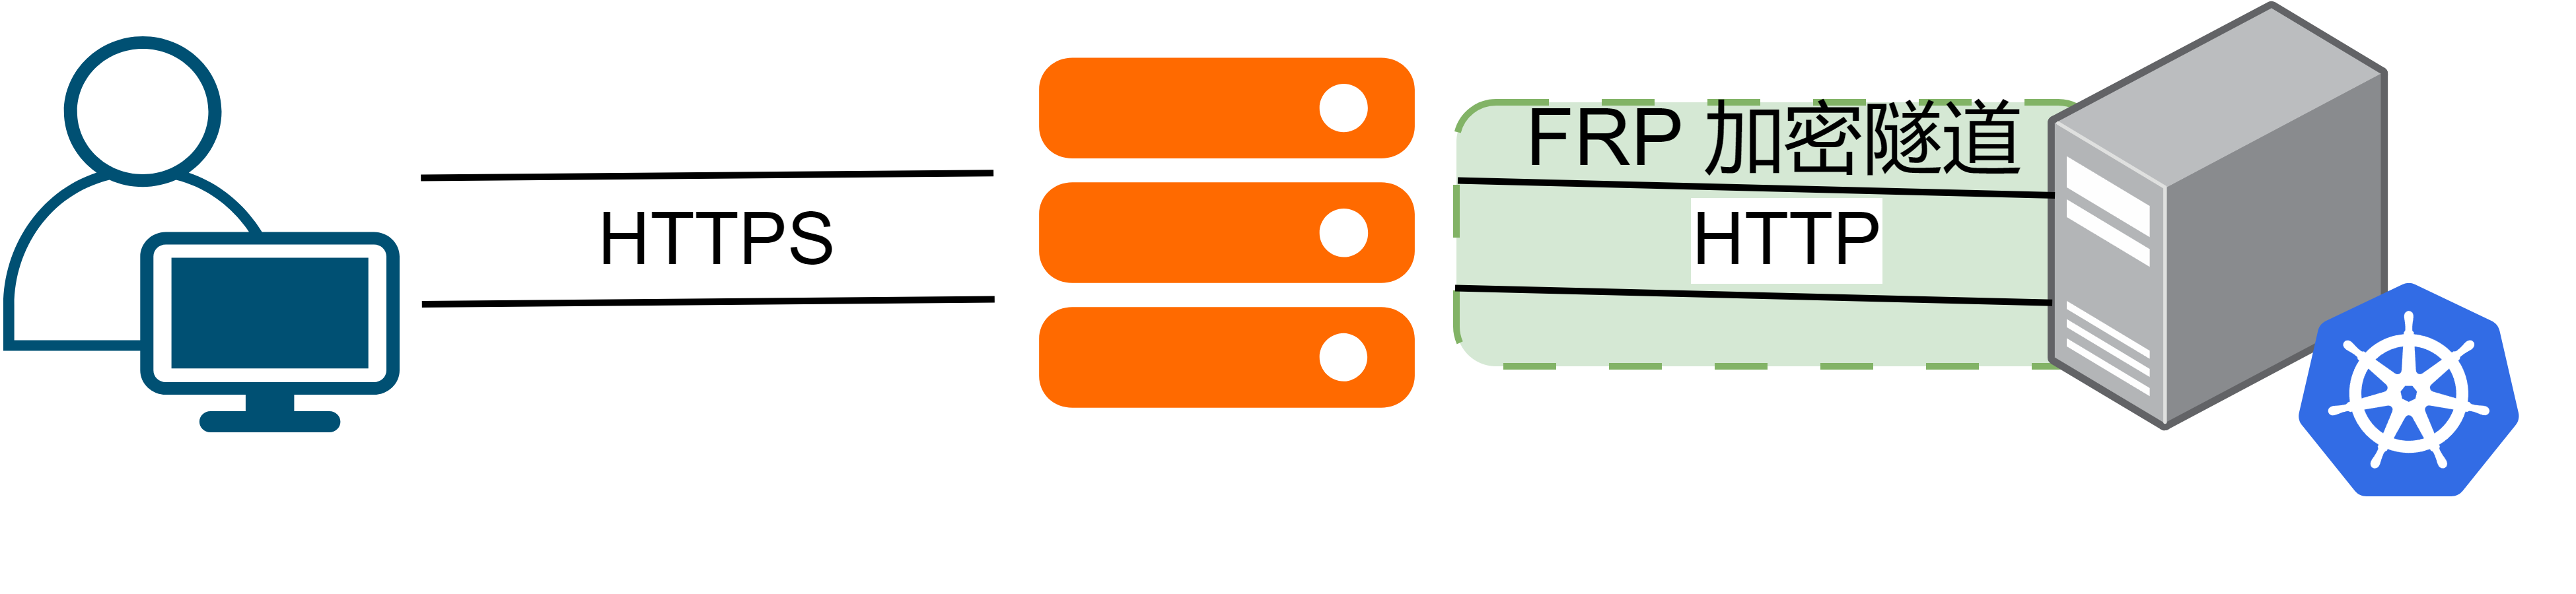
\includegraphics[width=1\textwidth]{assets/未命名绘图.drawio (4).png}
				\caption{其他平台采用http传输,容易被窃听}
			\end{figure}
		\end{minipage}\hspace{0.3cm}
		\begin{minipage}{0.45\linewidth}
			\begin{figure}[h]
				\centering
				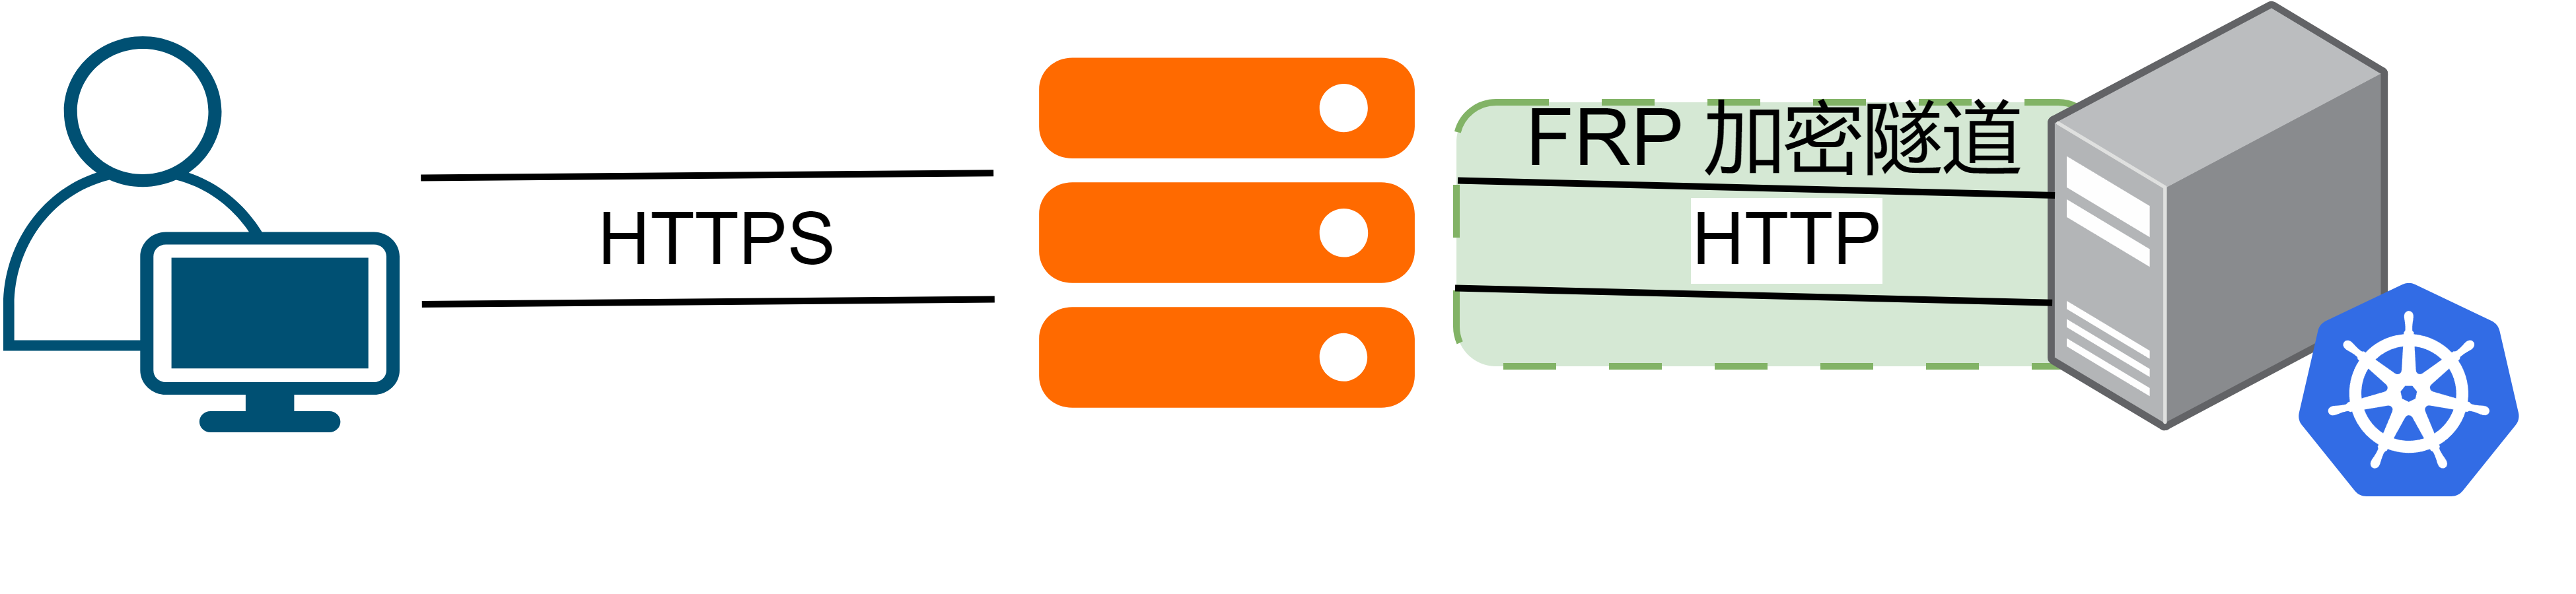
\includegraphics[width=1\textwidth]{assets/未命名绘图.drawio (4).png}
				\caption{铛铛支付平台采用https加密传输,保证数据安全}

			\end{figure}
		\end{minipage}%\hspace{0.1cm}
	\end{block}
\end{frame}


\begin{frame}{还有亿些项目亮点}
	\begin{itemize}
		\item
		      邮箱验证码
		\item
		      人机验证码
		\item
		      Jwt做登录状态
		\item
		      支持用户上传自己的头像和文件
		\item
		      全程日志记录
		\item
		      全自动参数校验
		\item
		      统一异常处理
		\item
		      使用Apifox记录接口信息
		\item
		      抵御Sql注入、Xss攻击
		\item
		      数据库用户密码加盐存储
		\item
		      Git 使用双分支开发,dev分支定时合并到主分支
		\item
		      Git提交粒度小
		\item
		      \ldots\ldots{}
	\end{itemize}
\end{frame}

%------------------------------------------------




% %------------------------------------------------

% \begin{frame}
%   \frametitle{设计思路}
%   \begin{block}{Slides with \LaTeX}
%     Beamer offers a lot of functions to create nice slides using \LaTeX.
%   \end{block}

%   \begin{block}{The basis}
%     内部使用以下主题
%     \begin{itemize}
%       \item split
%       \item whale
%       \item rounded
%       \item orchid
%     \end{itemize}
%   \end{block}
% \end{frame}
% %------------------------------------------------
% \begin{frame}
%   \frametitle{带数字列表}
%   \begin{enumerate}
%     \item This just shows the effect of the style
%     \item It is not a Beamer tutorial
%     \item Read the Beamer manual for more help
%     \item Contact me only concerning the style file
%   \end{enumerate}
% \end{frame}
% %------------------------------------------------
% \begin{frame}{块并列}
%   \begin{columns}
%     \begin{column}{0.5\textwidth}
%       \begin{block}{block1}
%         %\footnotesize{
%         \begin{enumerate}
%           \item item1
%                 \begin{itemize}
%                   \item  item1.1
%                 \end{itemize}
%           \item item2
%                 \begin{itemize}
%                   \item item2.1
%                 \end{itemize}
%           \item item3
%                 \begin{itemize}
%                   \item item3.1
%                 \end{itemize}
%         \end{enumerate}
%         %}    
%       \end{block}
%     \end{column}
%     \begin{column}{0.5\textwidth}
%       \begin{block}{block2}
%         %\footnotesize{
%         \begin{enumerate}
%           \item item1
%                 \begin{itemize}
%                   \item  item1.1
%                 \end{itemize}
%           \item item2
%                 \begin{itemize}
%                   \item item2.1
%                 \end{itemize}
%           \item item3
%                 \begin{itemize}
%                   \item item3.1
%                 \end{itemize}
%         \end{enumerate}
%         %}    
%       \end{block}
%     \end{column}
%   \end{columns}
% \end{frame}
% %------------------------------------------------

\begin{frame}{图片}
	\begin{minipage}{0.4\linewidth}
		\begin{figure}[h]
			\centering
			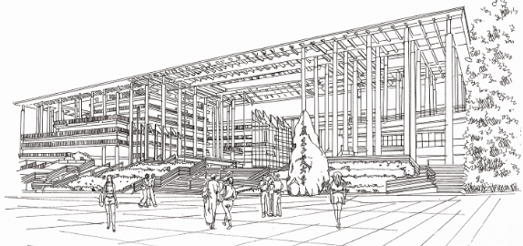
\includegraphics[height=.4\textheight]{res/GDUT-gate.png}
			\caption{GDUT}
		\end{figure}
	\end{minipage}\hspace{0.3cm}
	\begin{minipage}{0.45\linewidth}
		\begin{figure}[h]
			\centering
			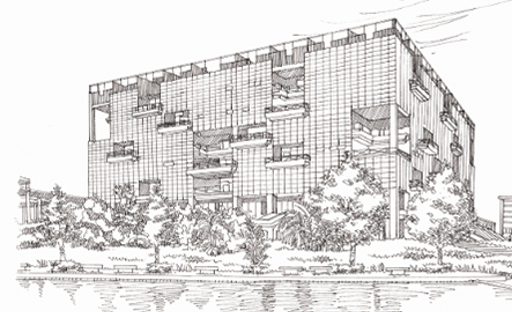
\includegraphics[height=.4\textheight]{res/GDUT-library.png}
			\caption{GDUT}
		\end{figure}
	\end{minipage}%\hspace{0.1cm}
\end{frame}
%------------------------------------------------

\begin{frame}[t]{块中多图}
	\begin{small}
		\begin{block}{多图比较与分析}
			\begin{minipage}{0.5\linewidth}
				\begin{figure}[h]
					\centering
					
\includegraphics[height=.2\textheight]{res/GDUT-logo.png}
					\caption{GDUT}
				\end{figure}
			\end{minipage}\hspace{0.1cm}
			\begin{minipage}{0.45\linewidth}
				\begin{figure}[h]
					\centering
					
\includegraphics[height=.2\textheight]{res/GDUT-logo_black.png}
					\caption{GDUT}
				\end{figure}
			\end{minipage}\hspace{0.1cm}
			%\medskip
			\begin{minipage}{0.5\linewidth}
				\begin{figure}[h]
					\centering
					
\includegraphics[height=.2\textheight]{res/GDUT-logo_white.png}
					\caption{GDUT}
				\end{figure}
			\end{minipage}\hspace{0.4cm}
			\begin{minipage}{0.4\linewidth}
				\begin{block}{}
					\begin{itemize}
						\scriptsize{
						\item ****************
						\item ****************
						\item ****************
						      }
					\end{itemize}
				\end{block}
			\end{minipage}
		\end{block}
	\end{small}
\end{frame}
%------------------------------------------------


% %------------------------------------------------
% \section{结论}
% %------------------------------------------------
% \begin{frame}
%   \subsection{  \frametitle{结论}}

%   \begin{itemize}
%     \item Easy to use
%     \item Good results
%   \end{itemize}
% \end{frame}
% %------------------------------------------------

% %------------------------------------------------
% \section{参考文献}
% %------------------------------------------------
% \begin{frame}
%   \frametitle{参考文献}
%   \begin{block}{}
%     \begin{minipage}{1\linewidth}
%       \scriptsize{
%         \begin{thebibliography}{99} % Beamer does not support BibTeX so references must be inserted manually as below
%           \bibitem{1} R. Sun, Y. Wang, L. Lyu, N. Cheng, S. Zhang, T. Yang, and X.Shen,“Delay-oriented caching strategies in d2d mobile networks,” \emph{IEEE Trans. Veh. Technol.}, vol. 69, no. 8, pp. 8529–8541, Aug. 2020.
%           \item Z. Su, Y. Hui, Q. Xu, T. Yang, J. Liu, and Y. Jia,“An edge caching scheme to distribute content in vehicular networks,” \emph{IEEE Trans. Veh. Technol.}, vol. 67, no. 6, pp. 5346–5356, Jun. 2018.
%           \item Q. Xu, Z. Su, Y. Wang, and K. Zhang,“Secure edge caching for layered multimedia contents in heterogeneous networks,” in \emph{Proc. IEEE Global Commun. Conf.}, Waikoloa, HI, USA, Dec. 2019, pp. 1–6.
%           \item B. Hu, L. Fang, X. Cheng, and L. Yang,“In-vehicle caching (iv-cache) via dynamic distributed storage relay ($d^2$sr) in vehicular networks,” \emph{IEEE Trans. Veh. Technol.}, vol. 68, no. 1, pp. 843–855, Jan. 2019.
%           \item C. Liu, K. Liu, S. Guo, R. Xie, V. C. S. Lee, and S. H. Son,“Adaptive offloading for time-critical tasks in heterogeneous internet of vehicles,” \emph{IEEE Internet Things J.}, vol. 7, no. 9, pp. 7999–8011, Sep. 2020.
%           \item J. Chen, H. Wu, P. Yang, F. Lyu, and X. Shen,“Cooperative edge caching with location-based and popular contents for vehicular networks,” \emph{IEEE Trans. Veh. Technol.}, vol. 69, no. 9, pp. 10291-10305, Jun. 2020.
%         \end{thebibliography}
%       }
%     \end{minipage}
%   \end{block}
% \end{frame}
% %------------------------------------------------


% %------------------------------------------------
\section{}

\begin{frame}
	\begin{block}{Ending}
		\Huge{\centerline{\emph{Thanks for Your Attention!}}}
		\Huge{\centerline{\emph{Q \& A ?}}}
	\end{block}

\end{frame}
%------------------------------------------------

\end{document}